\documentclass{whiteboard}
\begin{document}
\begin{frame}[plain,t]
\bbcover{Grafos}{Árvores: Travessias}{Prof. Edson Alves}{Faculdade UnB Gama}

\end{frame}
\begin{frame}[plain,t]
\begin{tikzpicture}
\node[draw,opacity=0] at (0, 0) {x};
\node[draw,opacity=0] at (14, 8) {x};

	\node[anchor=west] (title) at (0.0, 7.0) { \Large \bbbold{DFS em árvores} };
\end{tikzpicture}
\end{frame}
\begin{frame}[plain,t]
\begin{tikzpicture}
\node[draw,opacity=0] at (0, 0) {x};
\node[draw,opacity=0] at (14, 8) {x};

	\node[anchor=west] (title) at (0.0, 7.0) { \Large \bbbold{DFS em árvores} };

	\node[anchor=west] (a) at (1.0, 6.0) { $\star$ \bbtext{A estrutura das árvores simplifica a implementação da DFS} };

\end{tikzpicture}
\end{frame}
\begin{frame}[plain,t]
\begin{tikzpicture}
\node[draw,opacity=0] at (0, 0) {x};
\node[draw,opacity=0] at (14, 8) {x};

	\node[anchor=west] (title) at (0.0, 7.0) { \Large \bbbold{DFS em árvores} };

	\node[anchor=west] (a) at (1.0, 6.0) { $\star$ \bbtext{A estrutura das árvores simplifica a implementação da DFS} };


	\node[anchor=west] (b) at (1.0, 5.0) { $\star$ \bbtext{Por conta da ausência de ciclos, a DFS em árvores dispensa o registro dos} };

	\node[anchor=west] (b1) at (0.5, 4.5) { \bbtext{vértices já visitados} };


\end{tikzpicture}
\end{frame}
\begin{frame}[plain,t]
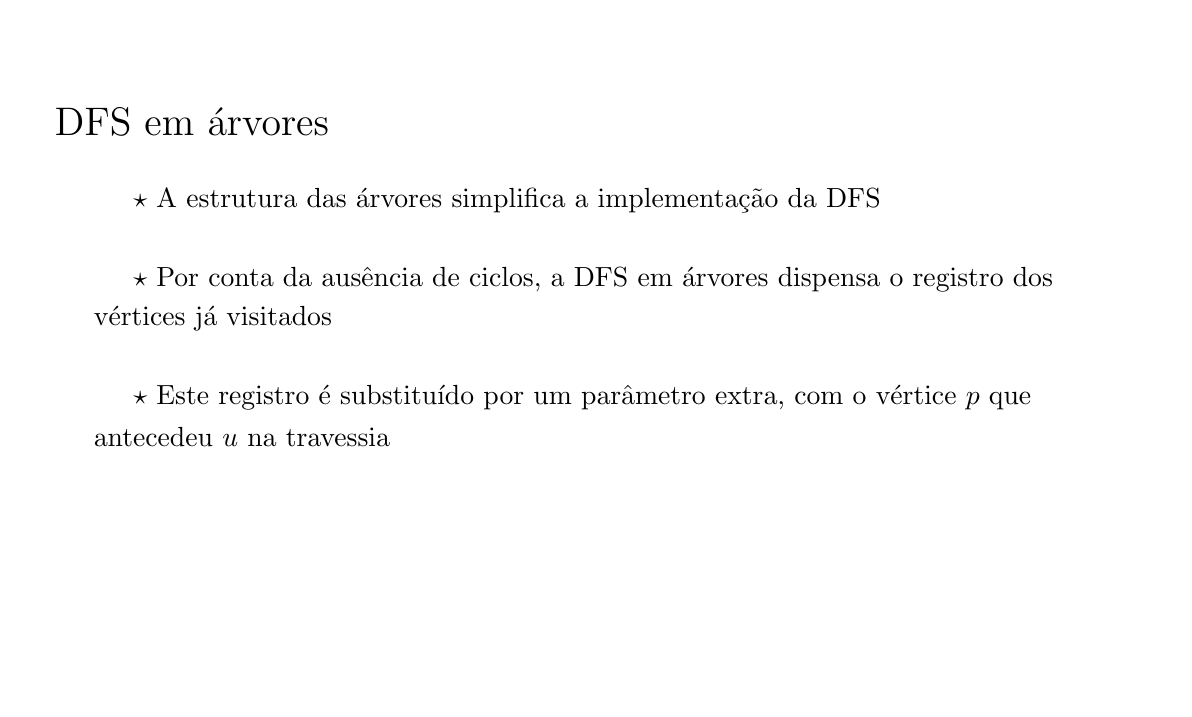
\begin{tikzpicture}
\node[draw,opacity=0] at (0, 0) {x};
\node[draw,opacity=0] at (14, 8) {x};

	\node[anchor=west] (title) at (0.0, 7.0) { \Large \bbbold{DFS em árvores} };

	\node[anchor=west] (a) at (1.0, 6.0) { $\star$ \bbtext{A estrutura das árvores simplifica a implementação da DFS} };


	\node[anchor=west] (b) at (1.0, 5.0) { $\star$ \bbtext{Por conta da ausência de ciclos, a DFS em árvores dispensa o registro dos} };

	\node[anchor=west] (b1) at (0.5, 4.5) { \bbtext{vértices já visitados} };



	\node[anchor=west] (c) at (1.0, 3.5) { $\star$ \bbtext{Este registro é substituído por um parâmetro extra, com o vértice $p$ que } };

	\node[anchor=west] (c1) at (0.5, 3.0) { \bbtext{antecedeu $u$ na travessia} };


\end{tikzpicture}
\end{frame}
\begin{frame}[plain,t]
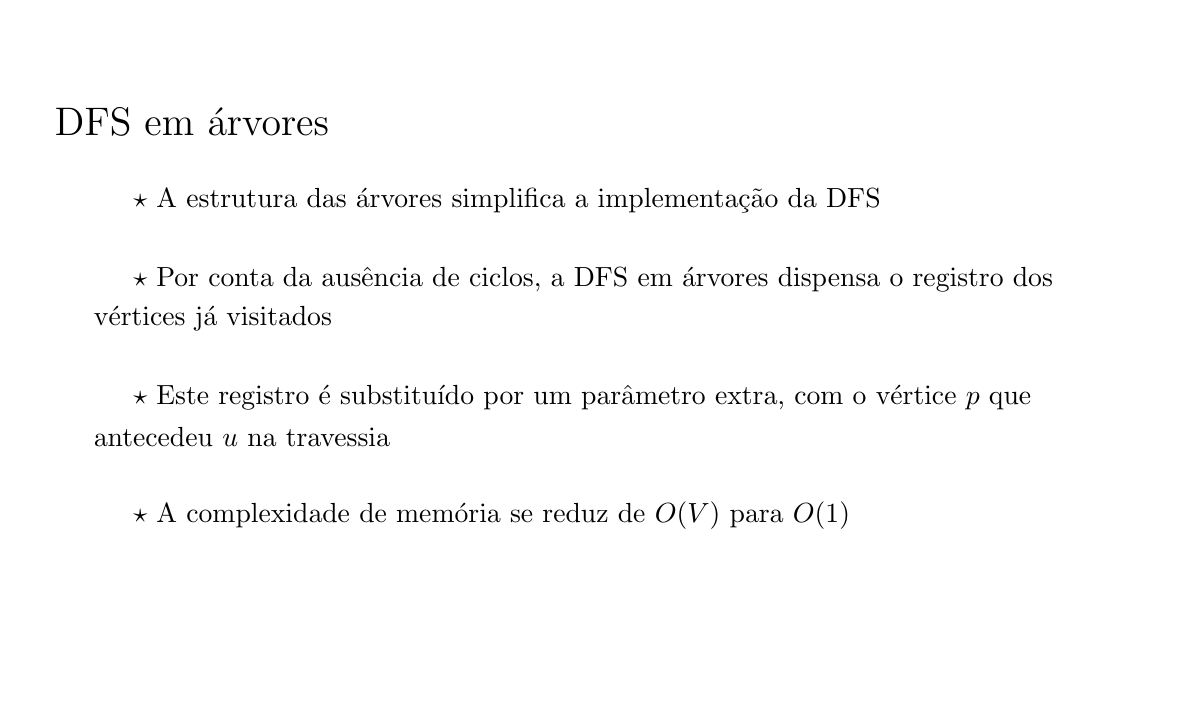
\begin{tikzpicture}
\node[draw,opacity=0] at (0, 0) {x};
\node[draw,opacity=0] at (14, 8) {x};

	\node[anchor=west] (title) at (0.0, 7.0) { \Large \bbbold{DFS em árvores} };

	\node[anchor=west] (a) at (1.0, 6.0) { $\star$ \bbtext{A estrutura das árvores simplifica a implementação da DFS} };


	\node[anchor=west] (b) at (1.0, 5.0) { $\star$ \bbtext{Por conta da ausência de ciclos, a DFS em árvores dispensa o registro dos} };

	\node[anchor=west] (b1) at (0.5, 4.5) { \bbtext{vértices já visitados} };



	\node[anchor=west] (c) at (1.0, 3.5) { $\star$ \bbtext{Este registro é substituído por um parâmetro extra, com o vértice $p$ que } };

	\node[anchor=west] (c1) at (0.5, 3.0) { \bbtext{antecedeu $u$ na travessia} };



	\node[anchor=west] (d) at (1.0, 2.0) { $\star$ \bbtext{A complexidade de memória se reduz de $O(V)$ para $O(1)$} };

\end{tikzpicture}
\end{frame}
\begin{frame}[plain,t]
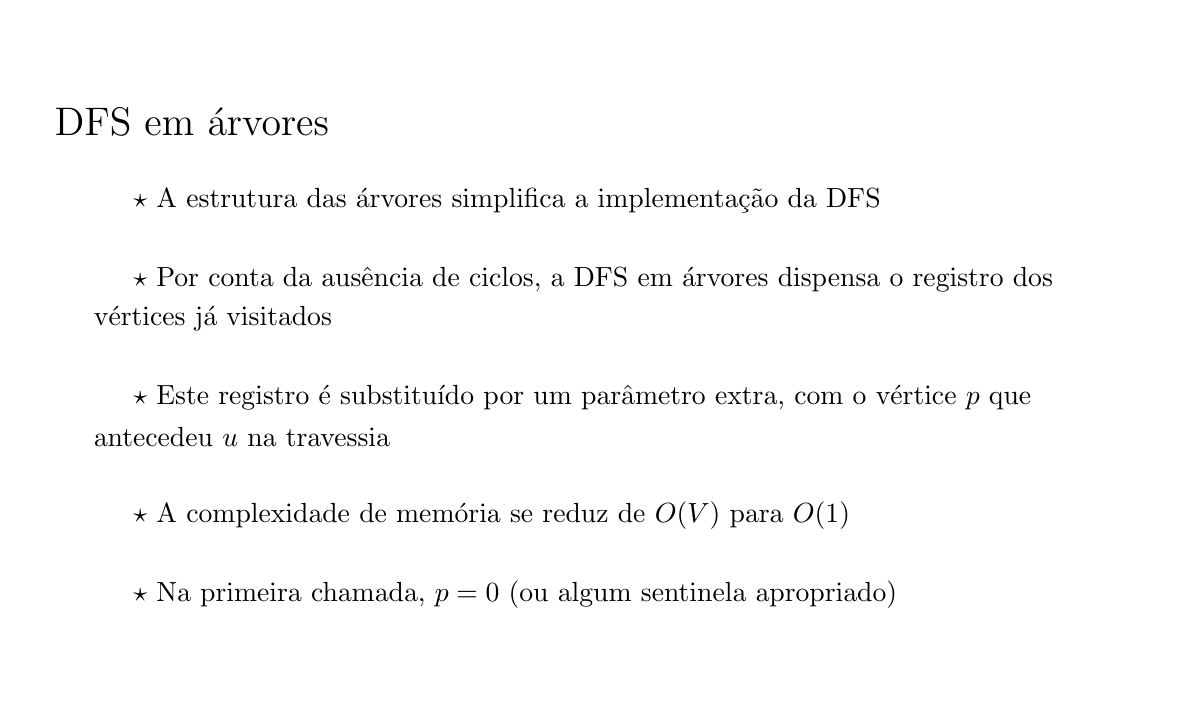
\begin{tikzpicture}
\node[draw,opacity=0] at (0, 0) {x};
\node[draw,opacity=0] at (14, 8) {x};

	\node[anchor=west] (title) at (0.0, 7.0) { \Large \bbbold{DFS em árvores} };

	\node[anchor=west] (a) at (1.0, 6.0) { $\star$ \bbtext{A estrutura das árvores simplifica a implementação da DFS} };


	\node[anchor=west] (b) at (1.0, 5.0) { $\star$ \bbtext{Por conta da ausência de ciclos, a DFS em árvores dispensa o registro dos} };

	\node[anchor=west] (b1) at (0.5, 4.5) { \bbtext{vértices já visitados} };



	\node[anchor=west] (c) at (1.0, 3.5) { $\star$ \bbtext{Este registro é substituído por um parâmetro extra, com o vértice $p$ que } };

	\node[anchor=west] (c1) at (0.5, 3.0) { \bbtext{antecedeu $u$ na travessia} };



	\node[anchor=west] (d) at (1.0, 2.0) { $\star$ \bbtext{A complexidade de memória se reduz de $O(V)$ para $O(1)$} };


	\node[anchor=west] (e) at (1.0, 1.0) { $\star$ \bbtext{Na primeira chamada, $p = 0$ (ou algum sentinela apropriado)} };


\end{tikzpicture}
\end{frame}
\begin{frame}[plain,t]

\inputcode{cpp}{codes/dfs.cpp}

\end{frame}
\begin{frame}[plain,t]
\begin{tikzpicture}
\node[draw,opacity=0] at (0, 0) {x};
\node[draw,opacity=0] at (14, 8) {x};

	\node[anchor=west] (title) at (0.0, 7.0) { \Large \bbbold{Números de nós na subárvore} };

\end{tikzpicture}
\end{frame}
\begin{frame}[plain,t]
\begin{tikzpicture}
\node[draw,opacity=0] at (0, 0) {x};
\node[draw,opacity=0] at (14, 8) {x};

	\node[anchor=west] (title) at (0.0, 7.0) { \Large \bbbold{Números de nós na subárvore} };


	\node[anchor=west] (a) at (1.0, 6.0) { $\star$ \bbtext{A DFS, em conjunto com técnicas de programação dinâmica, permite} };

	\node[anchor=west] (a1) at (0.5, 5.5) { \bbtext{computar em $O(N)$ algumas características da árvore} };

\end{tikzpicture}
\end{frame}
\begin{frame}[plain,t]

\begin{tikzpicture}
\node[draw,opacity=0] at (0, 0) {x};
\node[draw,opacity=0] at (14, 8) {x};

	\node[anchor=west] (title) at (0.0, 7.0) { \Large \bbbold{Números de nós na subárvore} };


	\node[anchor=west] (a) at (1.0, 6.0) { $\star$ \bbtext{A DFS, em conjunto com técnicas de programação dinâmica, permite} };

	\node[anchor=west] (a1) at (0.5, 5.5) { \bbtext{computar em $O(N)$ algumas características da árvore} };


	\node[anchor=west] (b) at (1.0, 4.5) { $\star$ \bbtext{Um exemplo seria o número de nós $\mathrm{nodes}[u]$ da subárvore cuja raiz é $u$} };


\end{tikzpicture}
\end{frame}
\begin{frame}[plain,t]
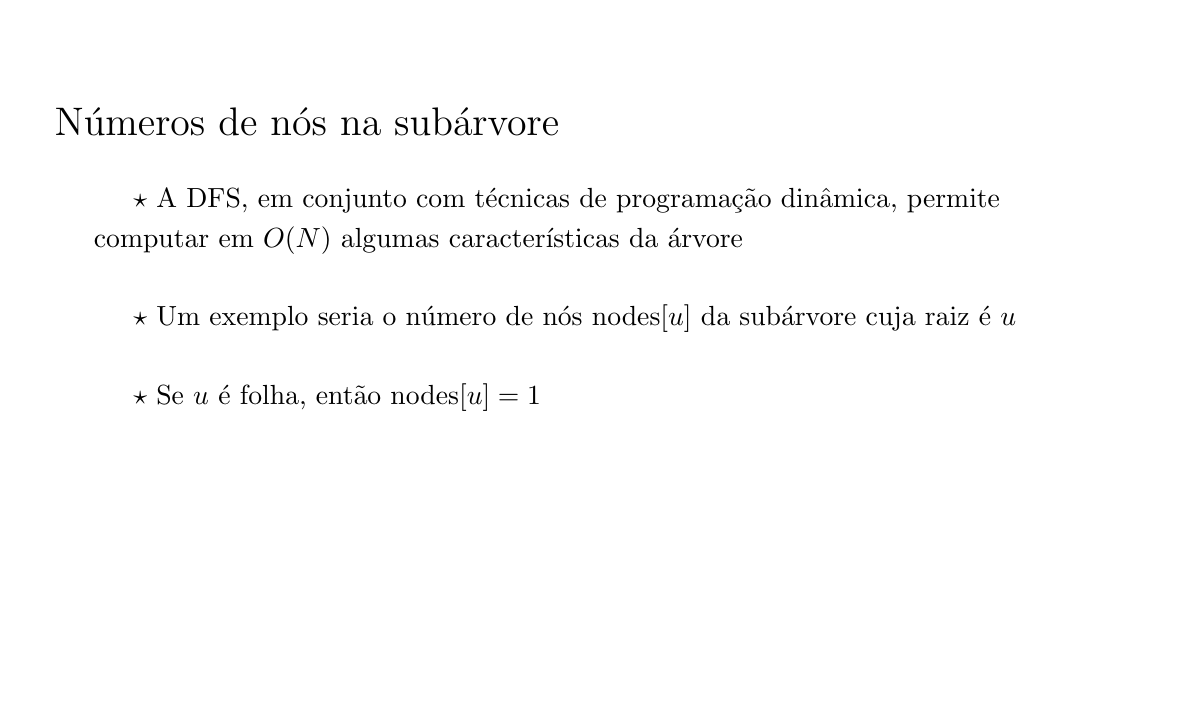
\begin{tikzpicture}
\node[draw,opacity=0] at (0, 0) {x};
\node[draw,opacity=0] at (14, 8) {x};

	\node[anchor=west] (title) at (0.0, 7.0) { \Large \bbbold{Números de nós na subárvore} };


	\node[anchor=west] (a) at (1.0, 6.0) { $\star$ \bbtext{A DFS, em conjunto com técnicas de programação dinâmica, permite} };

	\node[anchor=west] (a1) at (0.5, 5.5) { \bbtext{computar em $O(N)$ algumas características da árvore} };


	\node[anchor=west] (b) at (1.0, 4.5) { $\star$ \bbtext{Um exemplo seria o número de nós $\mathrm{nodes}[u]$ da subárvore cuja raiz é $u$} };



	\node[anchor=west] (c) at (1.0, 3.5) { $\star$ \bbtext{Se $u$ é folha, então $\mathrm{nodes}[u] = 1$} };

\end{tikzpicture}
\end{frame}
\begin{frame}[plain,t]
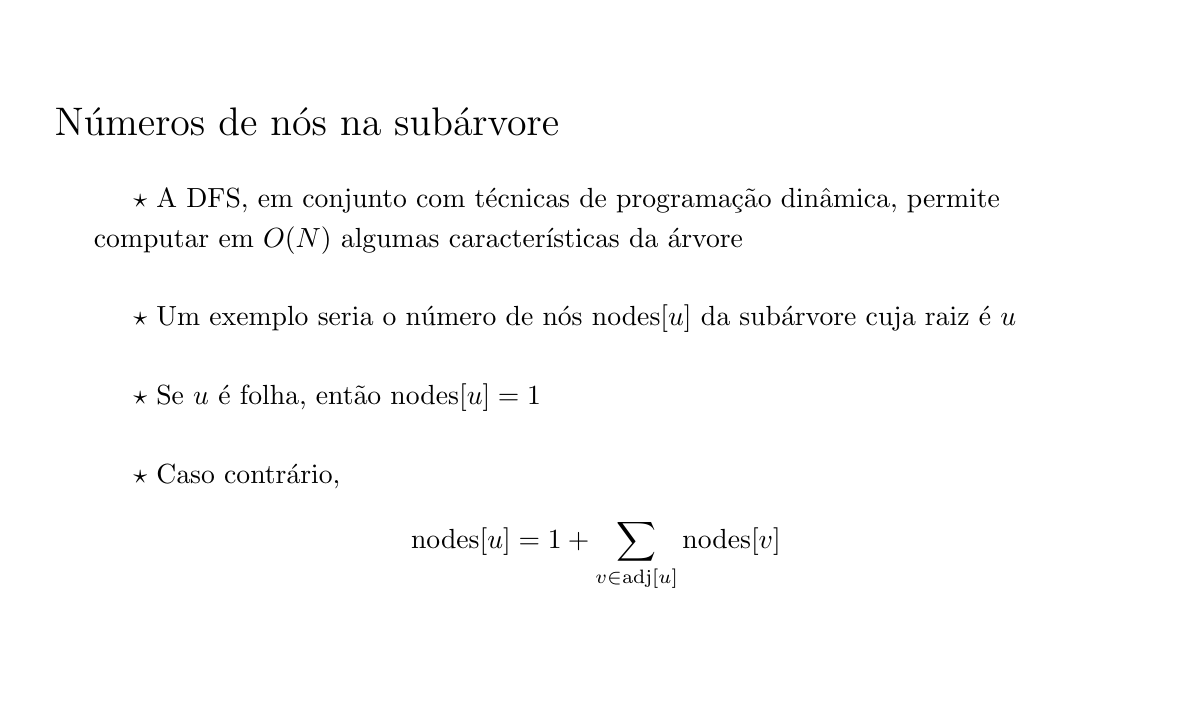
\begin{tikzpicture}
\node[draw,opacity=0] at (0, 0) {x};
\node[draw,opacity=0] at (14, 8) {x};

	\node[anchor=west] (title) at (0.0, 7.0) { \Large \bbbold{Números de nós na subárvore} };


	\node[anchor=west] (a) at (1.0, 6.0) { $\star$ \bbtext{A DFS, em conjunto com técnicas de programação dinâmica, permite} };

	\node[anchor=west] (a1) at (0.5, 5.5) { \bbtext{computar em $O(N)$ algumas características da árvore} };


	\node[anchor=west] (b) at (1.0, 4.5) { $\star$ \bbtext{Um exemplo seria o número de nós $\mathrm{nodes}[u]$ da subárvore cuja raiz é $u$} };



	\node[anchor=west] (c) at (1.0, 3.5) { $\star$ \bbtext{Se $u$ é folha, então $\mathrm{nodes}[u] = 1$} };


	\node[anchor=west] (d) at (1.0, 2.5) { $\star$ \bbtext{Caso contrário,} };

	\node[] (d1) at (7.0, 1.5) { $\displaystyle \mathrm{nodes}[u] = 1 + \sum_{v \in \mathrm{adj}[u]} \mathrm{nodes}[v]$ };

\end{tikzpicture}
\end{frame}
\begin{frame}[plain,t]
\begin{tikzpicture}
\node[draw,opacity=0] at (0, 0) {x};
\node[draw,opacity=0] at (14, 8) {x};

	\node[draw,very thick,circle] (node4) at (7.0, 7.0) { \bbtext{4} };

	\node[draw,very thick,circle] (node7) at (3.0, 5.0) { \bbtext{7} };

	\node[draw,very thick,circle] (node2) at (7.0, 5.0) { \bbtext{2} };

	\node[draw,very thick,circle] (node5) at (11.0, 5.0) { \bbtext{5} };

	\node[draw,very thick,circle] (node1) at (1.0, 3.0) { \bbtext{1} };

	\node[draw,very thick,circle] (node3) at (5.0, 3.0) { \bbtext{3} };

	\node[draw,very thick,circle] (node6) at (11.0, 3.0) { \bbtext{6} };

	\draw[thick](node4) to (node7);

	\draw[thick](node4) to (node2);

	\draw[thick](node4) to (node5);

	\draw[thick](node7) to (node1);

	\draw[thick](node7) to (node3);

	\draw[thick](node5) to (node6);

	\draw[] (4.0, 0.0) grid  (11.0, 1.0);

	\node[anchor=east] (text) at (3.9, 0.5) { $\mathrm{nodes}[u] = $ };

	\node[] (1) at (4.5, 1.5) { \bbtext{1} };

	\node[] (2) at (5.5, 1.5) { \bbtext{2} };

	\node[] (3) at (6.5, 1.5) { \bbtext{3} };

	\node[] (4) at (7.5, 1.5) { \bbtext{4} };

	\node[] (5) at (8.5, 1.5) { \bbtext{5} };

	\node[] (6) at (9.5, 1.5) { \bbtext{6} };

	\node[] (7) at (10.5, 1.5) { \bbtext{7} };

	\node[] (n1) at (4.5, 0.5) { \bbtext{-} };

	\node[] (n2) at (5.5, 0.5) { \bbtext{-} };

	\node[] (n3) at (6.5, 0.5) { \bbtext{-} };

	\node[] (n4) at (7.5, 0.5) { \bbtext{-} };

	\node[] (n5) at (8.5, 0.5) { \bbtext{-} };

	\node[] (n6) at (9.5, 0.5) { \bbtext{-} };

	\node[] (n7) at (10.5, 0.5) { \bbtext{-} };

\end{tikzpicture}
\end{frame}
\begin{frame}[plain,t]
\begin{tikzpicture}
\node[draw,opacity=0] at (0, 0) {x};
\node[draw,opacity=0] at (14, 8) {x};

	\node[draw,very thick,circle,fill=BBGreen] (node4) at (7.0, 7.0) { \bbtext{4} };

	\node[draw,very thick,circle] (node7) at (3.0, 5.0) { \bbtext{7} };

	\node[draw,very thick,circle] (node2) at (7.0, 5.0) { \bbtext{2} };

	\node[draw,very thick,circle] (node5) at (11.0, 5.0) { \bbtext{5} };

	\node[draw,very thick,circle] (node1) at (1.0, 3.0) { \bbtext{1} };

	\node[draw,very thick,circle] (node3) at (5.0, 3.0) { \bbtext{3} };

	\node[draw,very thick,circle] (node6) at (11.0, 3.0) { \bbtext{6} };

	\draw[thick](node4) to (node7);

	\draw[thick](node4) to (node2);

	\draw[thick](node4) to (node5);

	\draw[thick](node7) to (node1);

	\draw[thick](node7) to (node3);

	\draw[thick](node5) to (node6);

	\draw[] (4.0, 0.0) grid  (11.0, 1.0);

	\node[anchor=east] (text) at (3.9, 0.5) { $\mathrm{nodes}[u] = $ };

	\node[] (1) at (4.5, 1.5) { \bbtext{1} };

	\node[] (2) at (5.5, 1.5) { \bbtext{2} };

	\node[] (3) at (6.5, 1.5) { \bbtext{3} };

	\node[] (4) at (7.5, 1.5) { \bbtext{4} };

	\node[] (5) at (8.5, 1.5) { \bbtext{5} };

	\node[] (6) at (9.5, 1.5) { \bbtext{6} };

	\node[] (7) at (10.5, 1.5) { \bbtext{7} };

	\node[] (n1) at (4.5, 0.5) { \bbtext{-} };

	\node[] (n2) at (5.5, 0.5) { \bbtext{-} };

	\node[] (n3) at (6.5, 0.5) { \bbtext{-} };

	\node[] (n4) at (7.5, 0.5) { $\mathbf{1}$ };

	\node[] (n5) at (8.5, 0.5) { \bbtext{-} };

	\node[] (n6) at (9.5, 0.5) { \bbtext{-} };

	\node[] (n7) at (10.5, 0.5) { \bbtext{-} };


\end{tikzpicture}
\end{frame}
\begin{frame}[plain,t]
\begin{tikzpicture}
\node[draw,opacity=0] at (0, 0) {x};
\node[draw,opacity=0] at (14, 8) {x};

	\node[draw,very thick,circle,fill=BBGray] (node4) at (7.0, 7.0) { \bbtext{4} };

	\node[draw,very thick,circle,fill=BBGreen] (node7) at (3.0, 5.0) { \bbtext{7} };

	\node[draw,very thick,circle] (node2) at (7.0, 5.0) { \bbtext{2} };

	\node[draw,very thick,circle] (node5) at (11.0, 5.0) { \bbtext{5} };

	\node[draw,very thick,circle] (node1) at (1.0, 3.0) { \bbtext{1} };

	\node[draw,very thick,circle] (node3) at (5.0, 3.0) { \bbtext{3} };

	\node[draw,very thick,circle] (node6) at (11.0, 3.0) { \bbtext{6} };

	\draw[thick](node4) to (node7);

	\draw[thick](node4) to (node2);

	\draw[thick](node4) to (node5);

	\draw[thick](node7) to (node1);

	\draw[thick](node7) to (node3);

	\draw[thick](node5) to (node6);

	\draw[] (4.0, 0.0) grid  (11.0, 1.0);

	\node[anchor=east] (text) at (3.9, 0.5) { $\mathrm{nodes}[u] = $ };

	\node[] (1) at (4.5, 1.5) { \bbtext{1} };

	\node[] (2) at (5.5, 1.5) { \bbtext{2} };

	\node[] (3) at (6.5, 1.5) { \bbtext{3} };

	\node[] (4) at (7.5, 1.5) { \bbtext{4} };

	\node[] (5) at (8.5, 1.5) { \bbtext{5} };

	\node[] (6) at (9.5, 1.5) { \bbtext{6} };

	\node[] (7) at (10.5, 1.5) { \bbtext{7} };

	\node[] (n1) at (4.5, 0.5) { \bbtext{-} };

	\node[] (n2) at (5.5, 0.5) { \bbtext{-} };

	\node[] (n3) at (6.5, 0.5) { \bbtext{-} };

	\node[] (n4) at (7.5, 0.5) { ${1}$ };

	\node[] (n5) at (8.5, 0.5) { \bbtext{-} };

	\node[] (n6) at (9.5, 0.5) { \bbtext{-} };

	\node[] (n7) at (10.5, 0.5) { $\mathbf{1}$ };



\end{tikzpicture}
\end{frame}
\begin{frame}[plain,t]
\begin{tikzpicture}
\node[draw,opacity=0] at (0, 0) {x};
\node[draw,opacity=0] at (14, 8) {x};

	\node[draw,very thick,circle,fill=BBGray] (node4) at (7.0, 7.0) { \bbtext{4} };

	\node[draw,very thick,circle,fill=BBGray] (node7) at (3.0, 5.0) { \bbtext{7} };

	\node[draw,very thick,circle] (node2) at (7.0, 5.0) { \bbtext{2} };

	\node[draw,very thick,circle] (node5) at (11.0, 5.0) { \bbtext{5} };

	\node[draw,very thick,circle,fill=BBCyan] (node1) at (1.0, 3.0) { \bbtext{1} };

	\node[draw,very thick,circle] (node3) at (5.0, 3.0) { \bbtext{3} };

	\node[draw,very thick,circle] (node6) at (11.0, 3.0) { \bbtext{6} };

	\draw[thick](node4) to (node7);

	\draw[thick](node4) to (node2);

	\draw[thick](node4) to (node5);

	\draw[thick](node7) to (node1);

	\draw[thick](node7) to (node3);

	\draw[thick](node5) to (node6);

	\draw[] (4.0, 0.0) grid  (11.0, 1.0);

	\node[anchor=east] (text) at (3.9, 0.5) { $\mathrm{nodes}[u] = $ };

	\node[] (1) at (4.5, 1.5) { \bbtext{1} };

	\node[] (2) at (5.5, 1.5) { \bbtext{2} };

	\node[] (3) at (6.5, 1.5) { \bbtext{3} };

	\node[] (4) at (7.5, 1.5) { \bbtext{4} };

	\node[] (5) at (8.5, 1.5) { \bbtext{5} };

	\node[] (6) at (9.5, 1.5) { \bbtext{6} };

	\node[] (7) at (10.5, 1.5) { \bbtext{7} };

	\node[] (n1) at (4.5, 0.5) { $\mathbf{1}$ };

	\node[] (n2) at (5.5, 0.5) { \bbtext{-} };

	\node[] (n3) at (6.5, 0.5) { \bbtext{-} };

	\node[] (n4) at (7.5, 0.5) { ${1}$ };

	\node[] (n5) at (8.5, 0.5) { \bbtext{-} };

	\node[] (n6) at (9.5, 0.5) { \bbtext{-} };

	\node[] (n7) at (10.5, 0.5) { ${1}$ };




\end{tikzpicture}
\end{frame}
\begin{frame}[plain,t]
\begin{tikzpicture}
\node[draw,opacity=0] at (0, 0) {x};
\node[draw,opacity=0] at (14, 8) {x};

	\node[draw,very thick,circle,fill=BBGray] (node4) at (7.0, 7.0) { \bbtext{4} };

	\node[draw,very thick,circle,fill=BBGreen] (node7) at (3.0, 5.0) { \bbtext{7} };

	\node[draw,very thick,circle] (node2) at (7.0, 5.0) { \bbtext{2} };

	\node[draw,very thick,circle] (node5) at (11.0, 5.0) { \bbtext{5} };

	\node[draw,very thick,circle,fill=BBCyan] (node1) at (1.0, 3.0) { \bbtext{1} };

	\node[draw,very thick,circle] (node3) at (5.0, 3.0) { \bbtext{3} };

	\node[draw,very thick,circle] (node6) at (11.0, 3.0) { \bbtext{6} };

	\draw[thick](node4) to (node7);

	\draw[thick](node4) to (node2);

	\draw[thick](node4) to (node5);

	\draw[thick](node7) to (node1);

	\draw[thick](node7) to (node3);

	\draw[thick](node5) to (node6);

	\draw[] (4.0, 0.0) grid  (11.0, 1.0);

	\node[anchor=east] (text) at (3.9, 0.5) { $\mathrm{nodes}[u] = $ };

	\node[] (1) at (4.5, 1.5) { \bbtext{1} };

	\node[] (2) at (5.5, 1.5) { \bbtext{2} };

	\node[] (3) at (6.5, 1.5) { \bbtext{3} };

	\node[] (4) at (7.5, 1.5) { \bbtext{4} };

	\node[] (5) at (8.5, 1.5) { \bbtext{5} };

	\node[] (6) at (9.5, 1.5) { \bbtext{6} };

	\node[] (7) at (10.5, 1.5) { \bbtext{7} };

	\node[] (n1) at (4.5, 0.5) { ${1}$ };

	\node[] (n2) at (5.5, 0.5) { \bbtext{-} };

	\node[] (n3) at (6.5, 0.5) { \bbtext{-} };

	\node[] (n4) at (7.5, 0.5) { ${1}$ };

	\node[] (n5) at (8.5, 0.5) { \bbtext{-} };

	\node[] (n6) at (9.5, 0.5) { \bbtext{-} };

	\node[] (n7) at (10.5, 0.5) { $\mathbf{2}$ };





\end{tikzpicture}
\end{frame}
\begin{frame}[plain,t]
\begin{tikzpicture}
\node[draw,opacity=0] at (0, 0) {x};
\node[draw,opacity=0] at (14, 8) {x};

	\node[draw,very thick,circle,fill=BBGray] (node4) at (7.0, 7.0) { \bbtext{4} };

	\node[draw,very thick,circle,fill=BBGray] (node7) at (3.0, 5.0) { \bbtext{7} };

	\node[draw,very thick,circle] (node2) at (7.0, 5.0) { \bbtext{2} };

	\node[draw,very thick,circle] (node5) at (11.0, 5.0) { \bbtext{5} };

	\node[draw,very thick,circle,fill=BBCyan] (node1) at (1.0, 3.0) { \bbtext{1} };

	\node[draw,very thick,circle,fill=BBCyan] (node3) at (5.0, 3.0) { \bbtext{3} };

	\node[draw,very thick,circle] (node6) at (11.0, 3.0) { \bbtext{6} };

	\draw[thick](node4) to (node7);

	\draw[thick](node4) to (node2);

	\draw[thick](node4) to (node5);

	\draw[thick](node7) to (node1);

	\draw[thick](node7) to (node3);

	\draw[thick](node5) to (node6);

	\draw[] (4.0, 0.0) grid  (11.0, 1.0);

	\node[anchor=east] (text) at (3.9, 0.5) { $\mathrm{nodes}[u] = $ };

	\node[] (1) at (4.5, 1.5) { \bbtext{1} };

	\node[] (2) at (5.5, 1.5) { \bbtext{2} };

	\node[] (3) at (6.5, 1.5) { \bbtext{3} };

	\node[] (4) at (7.5, 1.5) { \bbtext{4} };

	\node[] (5) at (8.5, 1.5) { \bbtext{5} };

	\node[] (6) at (9.5, 1.5) { \bbtext{6} };

	\node[] (7) at (10.5, 1.5) { \bbtext{7} };

	\node[] (n1) at (4.5, 0.5) { ${1}$ };

	\node[] (n2) at (5.5, 0.5) { \bbtext{-} };

	\node[] (n3) at (6.5, 0.5) { $\mathbf{1}$ };

	\node[] (n4) at (7.5, 0.5) { ${1}$ };

	\node[] (n5) at (8.5, 0.5) { \bbtext{-} };

	\node[] (n6) at (9.5, 0.5) { \bbtext{-} };

	\node[] (n7) at (10.5, 0.5) { ${2}$ };






\end{tikzpicture}
\end{frame}
\begin{frame}[plain,t]
\begin{tikzpicture}
\node[draw,opacity=0] at (0, 0) {x};
\node[draw,opacity=0] at (14, 8) {x};

	\node[draw,very thick,circle,fill=BBGray] (node4) at (7.0, 7.0) { \bbtext{4} };

	\node[draw,very thick,circle,fill=BBCyan] (node7) at (3.0, 5.0) { \bbtext{7} };

	\node[draw,very thick,circle] (node2) at (7.0, 5.0) { \bbtext{2} };

	\node[draw,very thick,circle] (node5) at (11.0, 5.0) { \bbtext{5} };

	\node[draw,very thick,circle,fill=BBCyan] (node1) at (1.0, 3.0) { \bbtext{1} };

	\node[draw,very thick,circle,fill=BBCyan] (node3) at (5.0, 3.0) { \bbtext{3} };

	\node[draw,very thick,circle] (node6) at (11.0, 3.0) { \bbtext{6} };

	\draw[thick](node4) to (node7);

	\draw[thick](node4) to (node2);

	\draw[thick](node4) to (node5);

	\draw[thick](node7) to (node1);

	\draw[thick](node7) to (node3);

	\draw[thick](node5) to (node6);

	\draw[] (4.0, 0.0) grid  (11.0, 1.0);

	\node[anchor=east] (text) at (3.9, 0.5) { $\mathrm{nodes}[u] = $ };

	\node[] (1) at (4.5, 1.5) { \bbtext{1} };

	\node[] (2) at (5.5, 1.5) { \bbtext{2} };

	\node[] (3) at (6.5, 1.5) { \bbtext{3} };

	\node[] (4) at (7.5, 1.5) { \bbtext{4} };

	\node[] (5) at (8.5, 1.5) { \bbtext{5} };

	\node[] (6) at (9.5, 1.5) { \bbtext{6} };

	\node[] (7) at (10.5, 1.5) { \bbtext{7} };

	\node[] (n1) at (4.5, 0.5) { ${1}$ };

	\node[] (n2) at (5.5, 0.5) { \bbtext{-} };

	\node[] (n3) at (6.5, 0.5) { ${1}$ };

	\node[] (n4) at (7.5, 0.5) { ${1}$ };

	\node[] (n5) at (8.5, 0.5) { \bbtext{-} };

	\node[] (n6) at (9.5, 0.5) { \bbtext{-} };

	\node[] (n7) at (10.5, 0.5) { $\mathbf{3}$ };







\end{tikzpicture}
\end{frame}
\begin{frame}[plain,t]
\begin{tikzpicture}
\node[draw,opacity=0] at (0, 0) {x};
\node[draw,opacity=0] at (14, 8) {x};

	\node[draw,very thick,circle,fill=BBGreen] (node4) at (7.0, 7.0) { \bbtext{4} };

	\node[draw,very thick,circle,fill=BBCyan] (node7) at (3.0, 5.0) { \bbtext{7} };

	\node[draw,very thick,circle] (node2) at (7.0, 5.0) { \bbtext{2} };

	\node[draw,very thick,circle] (node5) at (11.0, 5.0) { \bbtext{5} };

	\node[draw,very thick,circle,fill=BBCyan] (node1) at (1.0, 3.0) { \bbtext{1} };

	\node[draw,very thick,circle,fill=BBCyan] (node3) at (5.0, 3.0) { \bbtext{3} };

	\node[draw,very thick,circle] (node6) at (11.0, 3.0) { \bbtext{6} };

	\draw[thick](node4) to (node7);

	\draw[thick](node4) to (node2);

	\draw[thick](node4) to (node5);

	\draw[thick](node7) to (node1);

	\draw[thick](node7) to (node3);

	\draw[thick](node5) to (node6);

	\draw[] (4.0, 0.0) grid  (11.0, 1.0);

	\node[anchor=east] (text) at (3.9, 0.5) { $\mathrm{nodes}[u] = $ };

	\node[] (1) at (4.5, 1.5) { \bbtext{1} };

	\node[] (2) at (5.5, 1.5) { \bbtext{2} };

	\node[] (3) at (6.5, 1.5) { \bbtext{3} };

	\node[] (4) at (7.5, 1.5) { \bbtext{4} };

	\node[] (5) at (8.5, 1.5) { \bbtext{5} };

	\node[] (6) at (9.5, 1.5) { \bbtext{6} };

	\node[] (7) at (10.5, 1.5) { \bbtext{7} };

	\node[] (n1) at (4.5, 0.5) { ${1}$ };

	\node[] (n2) at (5.5, 0.5) { \bbtext{-} };

	\node[] (n3) at (6.5, 0.5) { ${1}$ };

	\node[] (n4) at (7.5, 0.5) { $\mathbf{4}$ };

	\node[] (n5) at (8.5, 0.5) { \bbtext{-} };

	\node[] (n6) at (9.5, 0.5) { \bbtext{-} };

	\node[] (n7) at (10.5, 0.5) { ${3}$ };








\end{tikzpicture}
\end{frame}
\begin{frame}[plain,t]
\begin{tikzpicture}
\node[draw,opacity=0] at (0, 0) {x};
\node[draw,opacity=0] at (14, 8) {x};

	\node[draw,very thick,circle,fill=BBGray] (node4) at (7.0, 7.0) { \bbtext{4} };

	\node[draw,very thick,circle,fill=BBCyan] (node7) at (3.0, 5.0) { \bbtext{7} };

	\node[draw,very thick,circle,fill=BBCyan] (node2) at (7.0, 5.0) { \bbtext{2} };

	\node[draw,very thick,circle] (node5) at (11.0, 5.0) { \bbtext{5} };

	\node[draw,very thick,circle,fill=BBCyan] (node1) at (1.0, 3.0) { \bbtext{1} };

	\node[draw,very thick,circle,fill=BBCyan] (node3) at (5.0, 3.0) { \bbtext{3} };

	\node[draw,very thick,circle] (node6) at (11.0, 3.0) { \bbtext{6} };

	\draw[thick](node4) to (node7);

	\draw[thick](node4) to (node2);

	\draw[thick](node4) to (node5);

	\draw[thick](node7) to (node1);

	\draw[thick](node7) to (node3);

	\draw[thick](node5) to (node6);

	\draw[] (4.0, 0.0) grid  (11.0, 1.0);

	\node[anchor=east] (text) at (3.9, 0.5) { $\mathrm{nodes}[u] = $ };

	\node[] (1) at (4.5, 1.5) { \bbtext{1} };

	\node[] (2) at (5.5, 1.5) { \bbtext{2} };

	\node[] (3) at (6.5, 1.5) { \bbtext{3} };

	\node[] (4) at (7.5, 1.5) { \bbtext{4} };

	\node[] (5) at (8.5, 1.5) { \bbtext{5} };

	\node[] (6) at (9.5, 1.5) { \bbtext{6} };

	\node[] (7) at (10.5, 1.5) { \bbtext{7} };

	\node[] (n1) at (4.5, 0.5) { ${1}$ };

	\node[] (n2) at (5.5, 0.5) { $\mathbf{1}$ };

	\node[] (n3) at (6.5, 0.5) { ${1}$ };

	\node[] (n4) at (7.5, 0.5) { ${4}$ };

	\node[] (n5) at (8.5, 0.5) { \bbtext{-} };

	\node[] (n6) at (9.5, 0.5) { \bbtext{-} };

	\node[] (n7) at (10.5, 0.5) { ${3}$ };









\end{tikzpicture}
\end{frame}
\begin{frame}[plain,t]
\begin{tikzpicture}
\node[draw,opacity=0] at (0, 0) {x};
\node[draw,opacity=0] at (14, 8) {x};

	\node[draw,very thick,circle,fill=BBGreen] (node4) at (7.0, 7.0) { \bbtext{4} };

	\node[draw,very thick,circle,fill=BBCyan] (node7) at (3.0, 5.0) { \bbtext{7} };

	\node[draw,very thick,circle,fill=BBCyan] (node2) at (7.0, 5.0) { \bbtext{2} };

	\node[draw,very thick,circle] (node5) at (11.0, 5.0) { \bbtext{5} };

	\node[draw,very thick,circle,fill=BBCyan] (node1) at (1.0, 3.0) { \bbtext{1} };

	\node[draw,very thick,circle,fill=BBCyan] (node3) at (5.0, 3.0) { \bbtext{3} };

	\node[draw,very thick,circle] (node6) at (11.0, 3.0) { \bbtext{6} };

	\draw[thick](node4) to (node7);

	\draw[thick](node4) to (node2);

	\draw[thick](node4) to (node5);

	\draw[thick](node7) to (node1);

	\draw[thick](node7) to (node3);

	\draw[thick](node5) to (node6);

	\draw[] (4.0, 0.0) grid  (11.0, 1.0);

	\node[anchor=east] (text) at (3.9, 0.5) { $\mathrm{nodes}[u] = $ };

	\node[] (1) at (4.5, 1.5) { \bbtext{1} };

	\node[] (2) at (5.5, 1.5) { \bbtext{2} };

	\node[] (3) at (6.5, 1.5) { \bbtext{3} };

	\node[] (4) at (7.5, 1.5) { \bbtext{4} };

	\node[] (5) at (8.5, 1.5) { \bbtext{5} };

	\node[] (6) at (9.5, 1.5) { \bbtext{6} };

	\node[] (7) at (10.5, 1.5) { \bbtext{7} };

	\node[] (n1) at (4.5, 0.5) { ${1}$ };

	\node[] (n2) at (5.5, 0.5) { ${1}$ };

	\node[] (n3) at (6.5, 0.5) { ${1}$ };

	\node[] (n4) at (7.5, 0.5) { $\mathbf{5}$ };

	\node[] (n5) at (8.5, 0.5) { \bbtext{-} };

	\node[] (n6) at (9.5, 0.5) { \bbtext{-} };

	\node[] (n7) at (10.5, 0.5) { ${3}$ };










\end{tikzpicture}
\end{frame}
\begin{frame}[plain,t]
\begin{tikzpicture}
\node[draw,opacity=0] at (0, 0) {x};
\node[draw,opacity=0] at (14, 8) {x};

	\node[draw,very thick,circle,fill=BBGray] (node4) at (7.0, 7.0) { \bbtext{4} };

	\node[draw,very thick,circle,fill=BBCyan] (node7) at (3.0, 5.0) { \bbtext{7} };

	\node[draw,very thick,circle,fill=BBCyan] (node2) at (7.0, 5.0) { \bbtext{2} };

	\node[draw,very thick,circle,fill=BBGreen] (node5) at (11.0, 5.0) { \bbtext{5} };

	\node[draw,very thick,circle,fill=BBCyan] (node1) at (1.0, 3.0) { \bbtext{1} };

	\node[draw,very thick,circle,fill=BBCyan] (node3) at (5.0, 3.0) { \bbtext{3} };

	\node[draw,very thick,circle] (node6) at (11.0, 3.0) { \bbtext{6} };

	\draw[thick](node4) to (node7);

	\draw[thick](node4) to (node2);

	\draw[thick](node4) to (node5);

	\draw[thick](node7) to (node1);

	\draw[thick](node7) to (node3);

	\draw[thick](node5) to (node6);

	\draw[] (4.0, 0.0) grid  (11.0, 1.0);

	\node[anchor=east] (text) at (3.9, 0.5) { $\mathrm{nodes}[u] = $ };

	\node[] (1) at (4.5, 1.5) { \bbtext{1} };

	\node[] (2) at (5.5, 1.5) { \bbtext{2} };

	\node[] (3) at (6.5, 1.5) { \bbtext{3} };

	\node[] (4) at (7.5, 1.5) { \bbtext{4} };

	\node[] (5) at (8.5, 1.5) { \bbtext{5} };

	\node[] (6) at (9.5, 1.5) { \bbtext{6} };

	\node[] (7) at (10.5, 1.5) { \bbtext{7} };

	\node[] (n1) at (4.5, 0.5) { ${1}$ };

	\node[] (n2) at (5.5, 0.5) { ${1}$ };

	\node[] (n3) at (6.5, 0.5) { ${1}$ };

	\node[] (n4) at (7.5, 0.5) { ${5}$ };

	\node[] (n5) at (8.5, 0.5) { $\mathbf{1}$ };

	\node[] (n6) at (9.5, 0.5) { \bbtext{-} };

	\node[] (n7) at (10.5, 0.5) { ${3}$ };











\end{tikzpicture}
\end{frame}
\begin{frame}[plain,t]
\begin{tikzpicture}
\node[draw,opacity=0] at (0, 0) {x};
\node[draw,opacity=0] at (14, 8) {x};

	\node[draw,very thick,circle,fill=BBGray] (node4) at (7.0, 7.0) { \bbtext{4} };

	\node[draw,very thick,circle,fill=BBCyan] (node7) at (3.0, 5.0) { \bbtext{7} };

	\node[draw,very thick,circle,fill=BBCyan] (node2) at (7.0, 5.0) { \bbtext{2} };

	\node[draw,very thick,circle,fill=BBGray] (node5) at (11.0, 5.0) { \bbtext{5} };

	\node[draw,very thick,circle,fill=BBCyan] (node1) at (1.0, 3.0) { \bbtext{1} };

	\node[draw,very thick,circle,fill=BBCyan] (node3) at (5.0, 3.0) { \bbtext{3} };

	\node[draw,very thick,circle,fill=BBCyan] (node6) at (11.0, 3.0) { \bbtext{6} };

	\draw[thick](node4) to (node7);

	\draw[thick](node4) to (node2);

	\draw[thick](node4) to (node5);

	\draw[thick](node7) to (node1);

	\draw[thick](node7) to (node3);

	\draw[thick](node5) to (node6);

	\draw[] (4.0, 0.0) grid  (11.0, 1.0);

	\node[anchor=east] (text) at (3.9, 0.5) { $\mathrm{nodes}[u] = $ };

	\node[] (1) at (4.5, 1.5) { \bbtext{1} };

	\node[] (2) at (5.5, 1.5) { \bbtext{2} };

	\node[] (3) at (6.5, 1.5) { \bbtext{3} };

	\node[] (4) at (7.5, 1.5) { \bbtext{4} };

	\node[] (5) at (8.5, 1.5) { \bbtext{5} };

	\node[] (6) at (9.5, 1.5) { \bbtext{6} };

	\node[] (7) at (10.5, 1.5) { \bbtext{7} };

	\node[] (n1) at (4.5, 0.5) { ${1}$ };

	\node[] (n2) at (5.5, 0.5) { ${1}$ };

	\node[] (n3) at (6.5, 0.5) { ${1}$ };

	\node[] (n4) at (7.5, 0.5) { ${5}$ };

	\node[] (n5) at (8.5, 0.5) { ${1}$ };

	\node[] (n6) at (9.5, 0.5) { $\mathbf{1}$ };

	\node[] (n7) at (10.5, 0.5) { ${3}$ };












\end{tikzpicture}
\end{frame}
\begin{frame}[plain,t]
\begin{tikzpicture}
\node[draw,opacity=0] at (0, 0) {x};
\node[draw,opacity=0] at (14, 8) {x};

	\node[draw,very thick,circle,fill=BBGray] (node4) at (7.0, 7.0) { \bbtext{4} };

	\node[draw,very thick,circle,fill=BBCyan] (node7) at (3.0, 5.0) { \bbtext{7} };

	\node[draw,very thick,circle,fill=BBCyan] (node2) at (7.0, 5.0) { \bbtext{2} };

	\node[draw,very thick,circle,fill=BBCyan] (node5) at (11.0, 5.0) { \bbtext{5} };

	\node[draw,very thick,circle,fill=BBCyan] (node1) at (1.0, 3.0) { \bbtext{1} };

	\node[draw,very thick,circle,fill=BBCyan] (node3) at (5.0, 3.0) { \bbtext{3} };

	\node[draw,very thick,circle,fill=BBCyan] (node6) at (11.0, 3.0) { \bbtext{6} };

	\draw[thick](node4) to (node7);

	\draw[thick](node4) to (node2);

	\draw[thick](node4) to (node5);

	\draw[thick](node7) to (node1);

	\draw[thick](node7) to (node3);

	\draw[thick](node5) to (node6);

	\draw[] (4.0, 0.0) grid  (11.0, 1.0);

	\node[anchor=east] (text) at (3.9, 0.5) { $\mathrm{nodes}[u] = $ };

	\node[] (1) at (4.5, 1.5) { \bbtext{1} };

	\node[] (2) at (5.5, 1.5) { \bbtext{2} };

	\node[] (3) at (6.5, 1.5) { \bbtext{3} };

	\node[] (4) at (7.5, 1.5) { \bbtext{4} };

	\node[] (5) at (8.5, 1.5) { \bbtext{5} };

	\node[] (6) at (9.5, 1.5) { \bbtext{6} };

	\node[] (7) at (10.5, 1.5) { \bbtext{7} };

	\node[] (n1) at (4.5, 0.5) { ${1}$ };

	\node[] (n2) at (5.5, 0.5) { ${1}$ };

	\node[] (n3) at (6.5, 0.5) { ${1}$ };

	\node[] (n4) at (7.5, 0.5) { ${5}$ };

	\node[] (n5) at (8.5, 0.5) { $\mathbf{2}$ };

	\node[] (n6) at (9.5, 0.5) { ${1}$ };

	\node[] (n7) at (10.5, 0.5) { ${3}$ };













\end{tikzpicture}
\end{frame}
\begin{frame}[plain,t]
\begin{tikzpicture}
\node[draw,opacity=0] at (0, 0) {x};
\node[draw,opacity=0] at (14, 8) {x};

	\node[draw,very thick,circle,fill=BBCyan] (node4) at (7.0, 7.0) { \bbtext{4} };

	\node[draw,very thick,circle,fill=BBCyan] (node7) at (3.0, 5.0) { \bbtext{7} };

	\node[draw,very thick,circle,fill=BBCyan] (node2) at (7.0, 5.0) { \bbtext{2} };

	\node[draw,very thick,circle,fill=BBCyan] (node5) at (11.0, 5.0) { \bbtext{5} };

	\node[draw,very thick,circle,fill=BBCyan] (node1) at (1.0, 3.0) { \bbtext{1} };

	\node[draw,very thick,circle,fill=BBCyan] (node3) at (5.0, 3.0) { \bbtext{3} };

	\node[draw,very thick,circle,fill=BBCyan] (node6) at (11.0, 3.0) { \bbtext{6} };

	\draw[thick](node4) to (node7);

	\draw[thick](node4) to (node2);

	\draw[thick](node4) to (node5);

	\draw[thick](node7) to (node1);

	\draw[thick](node7) to (node3);

	\draw[thick](node5) to (node6);

	\draw[] (4.0, 0.0) grid  (11.0, 1.0);

	\node[anchor=east] (text) at (3.9, 0.5) { $\mathrm{nodes}[u] = $ };

	\node[] (1) at (4.5, 1.5) { \bbtext{1} };

	\node[] (2) at (5.5, 1.5) { \bbtext{2} };

	\node[] (3) at (6.5, 1.5) { \bbtext{3} };

	\node[] (4) at (7.5, 1.5) { \bbtext{4} };

	\node[] (5) at (8.5, 1.5) { \bbtext{5} };

	\node[] (6) at (9.5, 1.5) { \bbtext{6} };

	\node[] (7) at (10.5, 1.5) { \bbtext{7} };

	\node[] (n1) at (4.5, 0.5) { ${1}$ };

	\node[] (n2) at (5.5, 0.5) { ${1}$ };

	\node[] (n3) at (6.5, 0.5) { ${1}$ };

	\node[] (n4) at (7.5, 0.5) { $\mathbf{7}$ };

	\node[] (n5) at (8.5, 0.5) { ${2}$ };

	\node[] (n6) at (9.5, 0.5) { ${1}$ };

	\node[] (n7) at (10.5, 0.5) { ${3}$ };














\end{tikzpicture}
\end{frame}
\begin{frame}[plain,t]
\begin{tikzpicture}
\node[draw,opacity=0] at (0, 0) {x};
\node[draw,opacity=0] at (14, 8) {x};

	\node[draw,very thick,circle,fill=BBCyan] (node4) at (7.0, 7.0) { \bbtext{4} };

	\node[draw,very thick,circle,fill=BBCyan] (node7) at (3.0, 5.0) { \bbtext{7} };

	\node[draw,very thick,circle,fill=BBCyan] (node2) at (7.0, 5.0) { \bbtext{2} };

	\node[draw,very thick,circle,fill=BBCyan] (node5) at (11.0, 5.0) { \bbtext{5} };

	\node[draw,very thick,circle,fill=BBCyan] (node1) at (1.0, 3.0) { \bbtext{1} };

	\node[draw,very thick,circle,fill=BBCyan] (node3) at (5.0, 3.0) { \bbtext{3} };

	\node[draw,very thick,circle,fill=BBCyan] (node6) at (11.0, 3.0) { \bbtext{6} };

	\draw[thick](node4) to (node7);

	\draw[thick](node4) to (node2);

	\draw[thick](node4) to (node5);

	\draw[thick](node7) to (node1);

	\draw[thick](node7) to (node3);

	\draw[thick](node5) to (node6);

	\draw[] (4.0, 0.0) grid  (11.0, 1.0);

	\node[anchor=east] (text) at (3.9, 0.5) { $\mathrm{nodes}[u] = $ };

	\node[] (1) at (4.5, 1.5) { \bbtext{1} };

	\node[] (2) at (5.5, 1.5) { \bbtext{2} };

	\node[] (3) at (6.5, 1.5) { \bbtext{3} };

	\node[] (4) at (7.5, 1.5) { \bbtext{4} };

	\node[] (5) at (8.5, 1.5) { \bbtext{5} };

	\node[] (6) at (9.5, 1.5) { \bbtext{6} };

	\node[] (7) at (10.5, 1.5) { \bbtext{7} };

	\node[] (n1) at (4.5, 0.5) { ${1}$ };

	\node[] (n2) at (5.5, 0.5) { ${1}$ };

	\node[] (n3) at (6.5, 0.5) { ${1}$ };

	\node[] (n4) at (7.5, 0.5) { ${7}$ };

	\node[] (n5) at (8.5, 0.5) { ${2}$ };

	\node[] (n6) at (9.5, 0.5) { ${1}$ };

	\node[] (n7) at (10.5, 0.5) { ${3}$ };















\end{tikzpicture}
\end{frame}
\begin{frame}[plain,t]

\inputsnippet{cpp}{9}{28}{codes/nodes.cpp}

\end{frame}
\begin{frame}[plain,t]
\begin{tikzpicture}
\node[draw,opacity=0] at (0, 0) {x};
\node[draw,opacity=0] at (14, 8) {x};

	\node[anchor=west] (title) at (0.0, 7.0) { \Large \bbbold{Maior caminho até uma folha} };

\end{tikzpicture}
\end{frame}
\begin{frame}[plain,t]
\begin{tikzpicture}
\node[draw,opacity=0] at (0, 0) {x};
\node[draw,opacity=0] at (14, 8) {x};

	\node[anchor=west] (title) at (0.0, 7.0) { \Large \bbbold{Maior caminho até uma folha} };


	\node[anchor=west] (a) at (1.0, 6.0) { $\star$ \bbtext{Outra aplicação de DFS com DP é o cálculo do tamanho, em arestas, do } };

	\node[anchor=west] (a1) at (0.5, 5.5) { \bbtext{maior caminho $\mathrm{toLeaf}[u]$ de $u$ até uma folha} };

\end{tikzpicture}
\end{frame}
\begin{frame}[plain,t]
\begin{tikzpicture}
\node[draw,opacity=0] at (0, 0) {x};
\node[draw,opacity=0] at (14, 8) {x};

	\node[anchor=west] (title) at (0.0, 7.0) { \Large \bbbold{Maior caminho até uma folha} };


	\node[anchor=west] (a) at (1.0, 6.0) { $\star$ \bbtext{Outra aplicação de DFS com DP é o cálculo do tamanho, em arestas, do } };

	\node[anchor=west] (a1) at (0.5, 5.5) { \bbtext{maior caminho $\mathrm{toLeaf}[u]$ de $u$ até uma folha} };


	\node[anchor=west] (b) at (1.0, 4.5) { $\star$ \bbtext{Se $u$ for uma folha, então $\mathrm{toLeaf}[u] = 0$} };

\end{tikzpicture}
\end{frame}
\begin{frame}[plain,t]
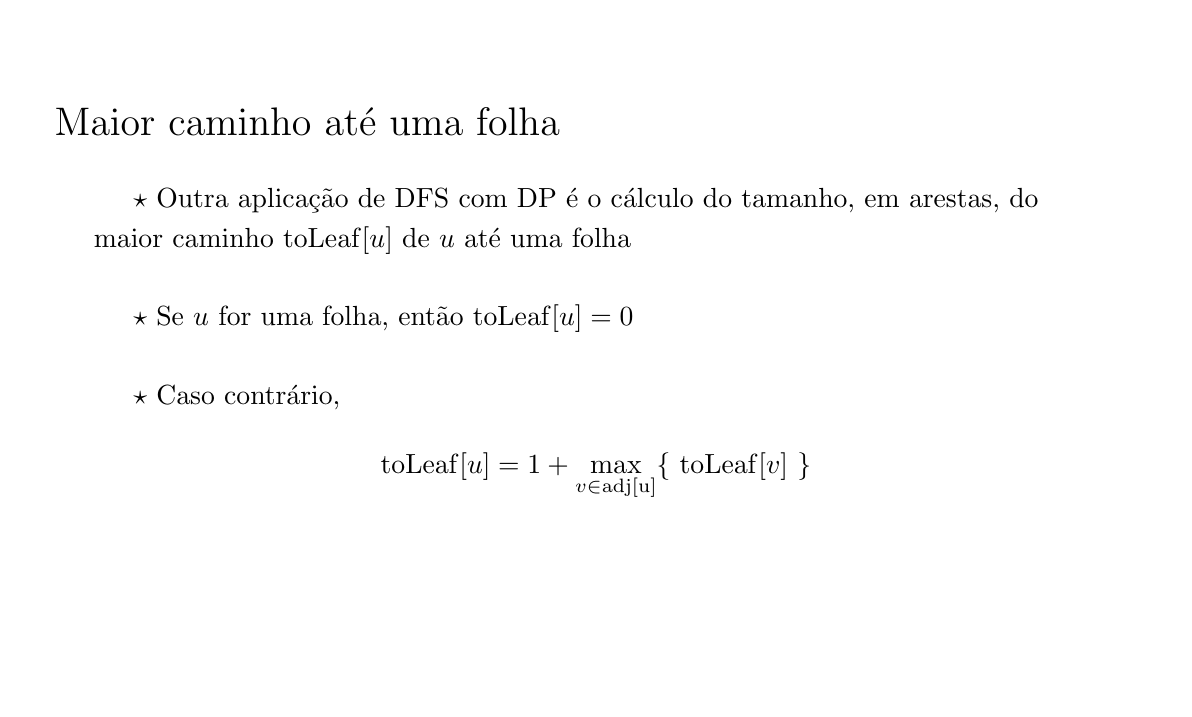
\begin{tikzpicture}
\node[draw,opacity=0] at (0, 0) {x};
\node[draw,opacity=0] at (14, 8) {x};

	\node[anchor=west] (title) at (0.0, 7.0) { \Large \bbbold{Maior caminho até uma folha} };


	\node[anchor=west] (a) at (1.0, 6.0) { $\star$ \bbtext{Outra aplicação de DFS com DP é o cálculo do tamanho, em arestas, do } };

	\node[anchor=west] (a1) at (0.5, 5.5) { \bbtext{maior caminho $\mathrm{toLeaf}[u]$ de $u$ até uma folha} };


	\node[anchor=west] (b) at (1.0, 4.5) { $\star$ \bbtext{Se $u$ for uma folha, então $\mathrm{toLeaf}[u] = 0$} };


	\node[anchor=west] (c) at (1.0, 3.5) { $\star$ \bbtext{Caso contrário,} };

	\node[] (c1) at (7.0, 2.5) { $\displaystyle \mathrm{toLeaf}[u] = 1 + \max_{v\in\mathrm{adj[u]}}\{\ \mathrm{toLeaf}[v]\ \}$ };

\end{tikzpicture}
\end{frame}
\begin{frame}[plain,t]
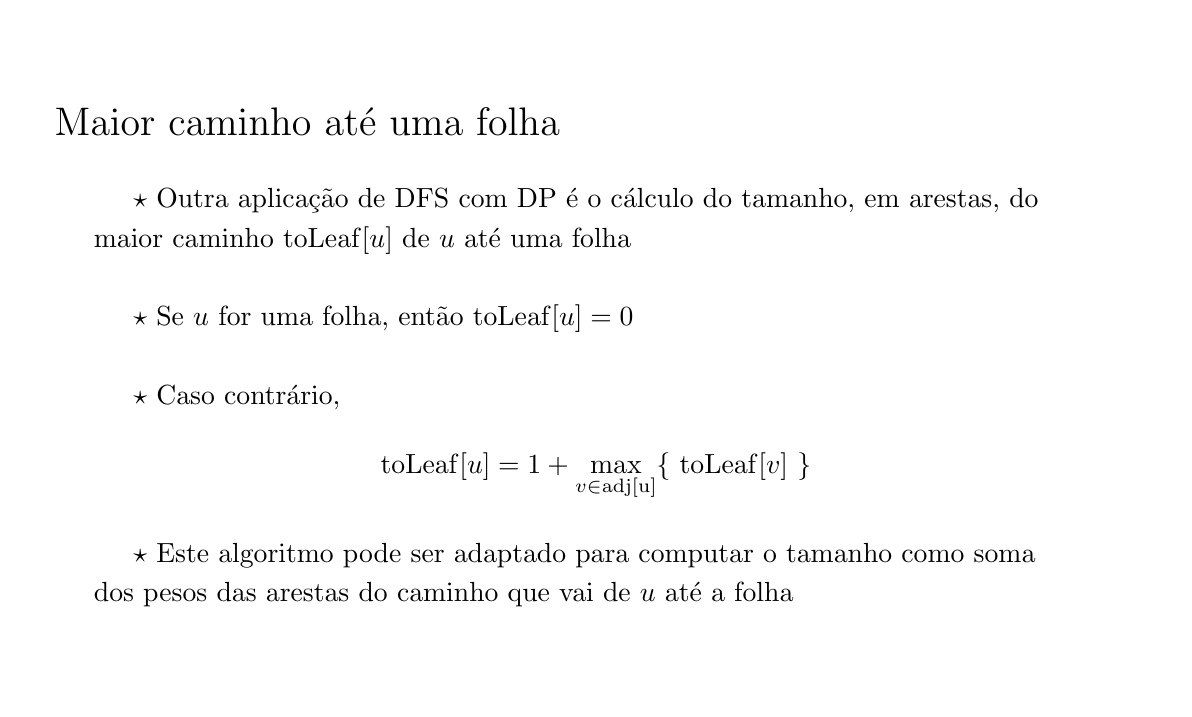
\begin{tikzpicture}
\node[draw,opacity=0] at (0, 0) {x};
\node[draw,opacity=0] at (14, 8) {x};

	\node[anchor=west] (title) at (0.0, 7.0) { \Large \bbbold{Maior caminho até uma folha} };


	\node[anchor=west] (a) at (1.0, 6.0) { $\star$ \bbtext{Outra aplicação de DFS com DP é o cálculo do tamanho, em arestas, do } };

	\node[anchor=west] (a1) at (0.5, 5.5) { \bbtext{maior caminho $\mathrm{toLeaf}[u]$ de $u$ até uma folha} };


	\node[anchor=west] (b) at (1.0, 4.5) { $\star$ \bbtext{Se $u$ for uma folha, então $\mathrm{toLeaf}[u] = 0$} };


	\node[anchor=west] (c) at (1.0, 3.5) { $\star$ \bbtext{Caso contrário,} };

	\node[] (c1) at (7.0, 2.5) { $\displaystyle \mathrm{toLeaf}[u] = 1 + \max_{v\in\mathrm{adj[u]}}\{\ \mathrm{toLeaf}[v]\ \}$ };


	\node[anchor=west] (d) at (1.0, 1.5) { $\star$ \bbtext{Este algoritmo pode ser adaptado para computar o tamanho como soma } };

	\node[anchor=west] (d1) at (0.5, 1.0) { \bbtext{dos pesos das arestas do caminho que vai de $u$ até a folha} };

\end{tikzpicture}
\end{frame}
\begin{frame}[plain,t]
\begin{tikzpicture}
\node[draw,opacity=0] at (0, 0) {x};
\node[draw,opacity=0] at (14, 8) {x};

	\node[draw,very thick,circle] (node4) at (6.0, 7.0) { \bbtext{4} };

	\node[draw,very thick,circle] (node7) at (10.0, 5.0) { \bbtext{7} };

	\node[draw,very thick,circle] (node2) at (6.0, 5.0) { \bbtext{2} };

	\node[draw,very thick,circle] (node5) at (2.0, 5.0) { \bbtext{5} };

	\node[draw,very thick,circle] (node1) at (8.0, 3.0) { \bbtext{1} };

	\node[draw,very thick,circle] (node3) at (12.0, 3.0) { \bbtext{3} };

	\node[draw,very thick,circle] (node6) at (2.0, 3.0) { \bbtext{6} };

	\draw[thick](node4) to (node7);

	\draw[thick](node4) to (node2);

	\draw[thick](node4) to (node5);

	\draw[thick](node7) to (node1);

	\draw[thick](node7) to (node3);

	\draw[thick](node5) to (node6);

	\draw[] (4.0, 0.0) grid  (11.0, 1.0);

	\node[anchor=east] (text) at (3.9, 0.5) { $\mathrm{toLeaf}[u] = $ };

	\node[] (1) at (4.5, 1.5) { \bbtext{1} };

	\node[] (2) at (5.5, 1.5) { \bbtext{2} };

	\node[] (3) at (6.5, 1.5) { \bbtext{3} };

	\node[] (4) at (7.5, 1.5) { \bbtext{4} };

	\node[] (5) at (8.5, 1.5) { \bbtext{5} };

	\node[] (6) at (9.5, 1.5) { \bbtext{6} };

	\node[] (7) at (10.5, 1.5) { \bbtext{7} };

	\node[] (n1) at (4.5, 0.5) { \bbtext{-} };

	\node[] (n2) at (5.5, 0.5) { \bbtext{-} };

	\node[] (n3) at (6.5, 0.5) { \bbtext{-} };

	\node[] (n4) at (7.5, 0.5) { \bbtext{-} };

	\node[] (n5) at (8.5, 0.5) { \bbtext{-} };

	\node[] (n6) at (9.5, 0.5) { \bbtext{-} };

	\node[] (n7) at (10.5, 0.5) { \bbtext{-} };

\end{tikzpicture}
\end{frame}
\begin{frame}[plain,t]
\begin{tikzpicture}
\node[draw,opacity=0] at (0, 0) {x};
\node[draw,opacity=0] at (14, 8) {x};

	\node[draw,very thick,circle,fill=BBGreen] (node4) at (6.0, 7.0) { \bbtext{4} };

	\node[draw,very thick,circle] (node7) at (10.0, 5.0) { \bbtext{7} };

	\node[draw,very thick,circle] (node2) at (6.0, 5.0) { \bbtext{2} };

	\node[draw,very thick,circle] (node5) at (2.0, 5.0) { \bbtext{5} };

	\node[draw,very thick,circle] (node1) at (8.0, 3.0) { \bbtext{1} };

	\node[draw,very thick,circle] (node3) at (12.0, 3.0) { \bbtext{3} };

	\node[draw,very thick,circle] (node6) at (2.0, 3.0) { \bbtext{6} };

	\draw[thick](node4) to (node7);

	\draw[thick](node4) to (node2);

	\draw[thick](node4) to (node5);

	\draw[thick](node7) to (node1);

	\draw[thick](node7) to (node3);

	\draw[thick](node5) to (node6);

	\draw[] (4.0, 0.0) grid  (11.0, 1.0);

	\node[anchor=east] (text) at (3.9, 0.5) { $\mathrm{toLeaf}[u] = $ };

	\node[] (1) at (4.5, 1.5) { \bbtext{1} };

	\node[] (2) at (5.5, 1.5) { \bbtext{2} };

	\node[] (3) at (6.5, 1.5) { \bbtext{3} };

	\node[] (4) at (7.5, 1.5) { \bbtext{4} };

	\node[] (5) at (8.5, 1.5) { \bbtext{5} };

	\node[] (6) at (9.5, 1.5) { \bbtext{6} };

	\node[] (7) at (10.5, 1.5) { \bbtext{7} };

	\node[] (n1) at (4.5, 0.5) { \bbtext{-} };

	\node[] (n2) at (5.5, 0.5) { \bbtext{-} };

	\node[] (n3) at (6.5, 0.5) { \bbtext{-} };

	\node[] (n4) at (7.5, 0.5) { \bbtext{-} };

	\node[] (n5) at (8.5, 0.5) { \bbtext{-} };

	\node[] (n6) at (9.5, 0.5) { \bbtext{-} };

	\node[] (n7) at (10.5, 0.5) { \bbtext{-} };



\end{tikzpicture}
\end{frame}
\begin{frame}[plain,t]
\begin{tikzpicture}
\node[draw,opacity=0] at (0, 0) {x};
\node[draw,opacity=0] at (14, 8) {x};

	\node[draw,very thick,circle,fill=BBGray] (node4) at (6.0, 7.0) { \bbtext{4} };

	\node[draw,very thick,circle] (node7) at (10.0, 5.0) { \bbtext{7} };

	\node[draw,very thick,circle] (node2) at (6.0, 5.0) { \bbtext{2} };

	\node[draw,very thick,circle,fill=BBGreen] (node5) at (2.0, 5.0) { \bbtext{5} };

	\node[draw,very thick,circle] (node1) at (8.0, 3.0) { \bbtext{1} };

	\node[draw,very thick,circle] (node3) at (12.0, 3.0) { \bbtext{3} };

	\node[draw,very thick,circle] (node6) at (2.0, 3.0) { \bbtext{6} };

	\draw[thick](node4) to (node7);

	\draw[thick](node4) to (node2);

	\draw[thick](node4) to (node5);

	\draw[thick](node7) to (node1);

	\draw[thick](node7) to (node3);

	\draw[thick](node5) to (node6);

	\draw[] (4.0, 0.0) grid  (11.0, 1.0);

	\node[anchor=east] (text) at (3.9, 0.5) { $\mathrm{toLeaf}[u] = $ };

	\node[] (1) at (4.5, 1.5) { \bbtext{1} };

	\node[] (2) at (5.5, 1.5) { \bbtext{2} };

	\node[] (3) at (6.5, 1.5) { \bbtext{3} };

	\node[] (4) at (7.5, 1.5) { \bbtext{4} };

	\node[] (5) at (8.5, 1.5) { \bbtext{5} };

	\node[] (6) at (9.5, 1.5) { \bbtext{6} };

	\node[] (7) at (10.5, 1.5) { \bbtext{7} };

	\node[] (n1) at (4.5, 0.5) { \bbtext{-} };

	\node[] (n2) at (5.5, 0.5) { \bbtext{-} };

	\node[] (n3) at (6.5, 0.5) { \bbtext{-} };

	\node[] (n4) at (7.5, 0.5) { \bbtext{-} };

	\node[] (n5) at (8.5, 0.5) { \bbtext{-} };

	\node[] (n6) at (9.5, 0.5) { \bbtext{-} };

	\node[] (n7) at (10.5, 0.5) { \bbtext{-} };





\end{tikzpicture}
\end{frame}
\begin{frame}[plain,t]
\begin{tikzpicture}
\node[draw,opacity=0] at (0, 0) {x};
\node[draw,opacity=0] at (14, 8) {x};

	\node[draw,very thick,circle,fill=BBGray] (node4) at (6.0, 7.0) { \bbtext{4} };

	\node[draw,very thick,circle] (node7) at (10.0, 5.0) { \bbtext{7} };

	\node[draw,very thick,circle] (node2) at (6.0, 5.0) { \bbtext{2} };

	\node[draw,very thick,circle,fill=BBGray] (node5) at (2.0, 5.0) { \bbtext{5} };

	\node[draw,very thick,circle] (node1) at (8.0, 3.0) { \bbtext{1} };

	\node[draw,very thick,circle] (node3) at (12.0, 3.0) { \bbtext{3} };

	\node[draw,very thick,circle,fill=BBCyan] (node6) at (2.0, 3.0) { \bbtext{6} };

	\draw[thick](node4) to (node7);

	\draw[thick](node4) to (node2);

	\draw[thick](node4) to (node5);

	\draw[thick](node7) to (node1);

	\draw[thick](node7) to (node3);

	\draw[thick](node5) to (node6);

	\draw[] (4.0, 0.0) grid  (11.0, 1.0);

	\node[anchor=east] (text) at (3.9, 0.5) { $\mathrm{toLeaf}[u] = $ };

	\node[] (1) at (4.5, 1.5) { \bbtext{1} };

	\node[] (2) at (5.5, 1.5) { \bbtext{2} };

	\node[] (3) at (6.5, 1.5) { \bbtext{3} };

	\node[] (4) at (7.5, 1.5) { \bbtext{4} };

	\node[] (5) at (8.5, 1.5) { \bbtext{5} };

	\node[] (6) at (9.5, 1.5) { \bbtext{6} };

	\node[] (7) at (10.5, 1.5) { \bbtext{7} };

	\node[] (n1) at (4.5, 0.5) { \bbtext{-} };

	\node[] (n2) at (5.5, 0.5) { \bbtext{-} };

	\node[] (n3) at (6.5, 0.5) { \bbtext{-} };

	\node[] (n4) at (7.5, 0.5) { \bbtext{-} };

	\node[] (n5) at (8.5, 0.5) { \bbtext{-} };

	\node[] (n6) at (9.5, 0.5) { $\mathbf{0}$ };

	\node[] (n7) at (10.5, 0.5) { \bbtext{-} };








\end{tikzpicture}
\end{frame}
\begin{frame}[plain,t]
\begin{tikzpicture}
\node[draw,opacity=0] at (0, 0) {x};
\node[draw,opacity=0] at (14, 8) {x};

	\node[draw,very thick,circle,fill=BBGray] (node4) at (6.0, 7.0) { \bbtext{4} };

	\node[draw,very thick,circle] (node7) at (10.0, 5.0) { \bbtext{7} };

	\node[draw,very thick,circle] (node2) at (6.0, 5.0) { \bbtext{2} };

	\node[draw,very thick,circle,fill=BBCyan] (node5) at (2.0, 5.0) { \bbtext{5} };

	\node[draw,very thick,circle] (node1) at (8.0, 3.0) { \bbtext{1} };

	\node[draw,very thick,circle] (node3) at (12.0, 3.0) { \bbtext{3} };

	\node[draw,very thick,circle,fill=BBCyan] (node6) at (2.0, 3.0) { \bbtext{6} };

	\draw[thick](node4) to (node7);

	\draw[thick](node4) to (node2);

	\draw[thick](node4) to (node5);

	\draw[thick](node7) to (node1);

	\draw[thick](node7) to (node3);

	\draw[thick](node5) to (node6);

	\draw[] (4.0, 0.0) grid  (11.0, 1.0);

	\node[anchor=east] (text) at (3.9, 0.5) { $\mathrm{toLeaf}[u] = $ };

	\node[] (1) at (4.5, 1.5) { \bbtext{1} };

	\node[] (2) at (5.5, 1.5) { \bbtext{2} };

	\node[] (3) at (6.5, 1.5) { \bbtext{3} };

	\node[] (4) at (7.5, 1.5) { \bbtext{4} };

	\node[] (5) at (8.5, 1.5) { \bbtext{5} };

	\node[] (6) at (9.5, 1.5) { \bbtext{6} };

	\node[] (7) at (10.5, 1.5) { \bbtext{7} };

	\node[] (n1) at (4.5, 0.5) { \bbtext{-} };

	\node[] (n2) at (5.5, 0.5) { \bbtext{-} };

	\node[] (n3) at (6.5, 0.5) { \bbtext{-} };

	\node[] (n4) at (7.5, 0.5) { \bbtext{-} };

	\node[] (n5) at (8.5, 0.5) { $\mathbf{1}$ };

	\node[] (n6) at (9.5, 0.5) { ${0}$ };

	\node[] (n7) at (10.5, 0.5) { \bbtext{-} };











\end{tikzpicture}
\end{frame}
\begin{frame}[plain,t]
\begin{tikzpicture}
\node[draw,opacity=0] at (0, 0) {x};
\node[draw,opacity=0] at (14, 8) {x};

	\node[draw,very thick,circle,fill=BBGreen] (node4) at (6.0, 7.0) { \bbtext{4} };

	\node[draw,very thick,circle] (node7) at (10.0, 5.0) { \bbtext{7} };

	\node[draw,very thick,circle] (node2) at (6.0, 5.0) { \bbtext{2} };

	\node[draw,very thick,circle,fill=BBCyan] (node5) at (2.0, 5.0) { \bbtext{5} };

	\node[draw,very thick,circle] (node1) at (8.0, 3.0) { \bbtext{1} };

	\node[draw,very thick,circle] (node3) at (12.0, 3.0) { \bbtext{3} };

	\node[draw,very thick,circle,fill=BBCyan] (node6) at (2.0, 3.0) { \bbtext{6} };

	\draw[thick](node4) to (node7);

	\draw[thick](node4) to (node2);

	\draw[thick](node4) to (node5);

	\draw[thick](node7) to (node1);

	\draw[thick](node7) to (node3);

	\draw[thick](node5) to (node6);

	\draw[] (4.0, 0.0) grid  (11.0, 1.0);

	\node[anchor=east] (text) at (3.9, 0.5) { $\mathrm{toLeaf}[u] = $ };

	\node[] (1) at (4.5, 1.5) { \bbtext{1} };

	\node[] (2) at (5.5, 1.5) { \bbtext{2} };

	\node[] (3) at (6.5, 1.5) { \bbtext{3} };

	\node[] (4) at (7.5, 1.5) { \bbtext{4} };

	\node[] (5) at (8.5, 1.5) { \bbtext{5} };

	\node[] (6) at (9.5, 1.5) { \bbtext{6} };

	\node[] (7) at (10.5, 1.5) { \bbtext{7} };

	\node[] (n1) at (4.5, 0.5) { \bbtext{-} };

	\node[] (n2) at (5.5, 0.5) { \bbtext{-} };

	\node[] (n3) at (6.5, 0.5) { \bbtext{-} };

	\node[] (n4) at (7.5, 0.5) { $\mathbf{2}$ };

	\node[] (n5) at (8.5, 0.5) { ${1}$ };

	\node[] (n6) at (9.5, 0.5) { ${0}$ };

	\node[] (n7) at (10.5, 0.5) { \bbtext{-} };














\end{tikzpicture}
\end{frame}
\begin{frame}[plain,t]
\begin{tikzpicture}
\node[draw,opacity=0] at (0, 0) {x};
\node[draw,opacity=0] at (14, 8) {x};

	\node[draw,very thick,circle,fill=BBGray] (node4) at (6.0, 7.0) { \bbtext{4} };

	\node[draw,very thick,circle] (node7) at (10.0, 5.0) { \bbtext{7} };

	\node[draw,very thick,circle,fill=BBCyan] (node2) at (6.0, 5.0) { \bbtext{2} };

	\node[draw,very thick,circle,fill=BBCyan] (node5) at (2.0, 5.0) { \bbtext{5} };

	\node[draw,very thick,circle] (node1) at (8.0, 3.0) { \bbtext{1} };

	\node[draw,very thick,circle] (node3) at (12.0, 3.0) { \bbtext{3} };

	\node[draw,very thick,circle,fill=BBCyan] (node6) at (2.0, 3.0) { \bbtext{6} };

	\draw[thick](node4) to (node7);

	\draw[thick](node4) to (node2);

	\draw[thick](node4) to (node5);

	\draw[thick](node7) to (node1);

	\draw[thick](node7) to (node3);

	\draw[thick](node5) to (node6);

	\draw[] (4.0, 0.0) grid  (11.0, 1.0);

	\node[anchor=east] (text) at (3.9, 0.5) { $\mathrm{toLeaf}[u] = $ };

	\node[] (1) at (4.5, 1.5) { \bbtext{1} };

	\node[] (2) at (5.5, 1.5) { \bbtext{2} };

	\node[] (3) at (6.5, 1.5) { \bbtext{3} };

	\node[] (4) at (7.5, 1.5) { \bbtext{4} };

	\node[] (5) at (8.5, 1.5) { \bbtext{5} };

	\node[] (6) at (9.5, 1.5) { \bbtext{6} };

	\node[] (7) at (10.5, 1.5) { \bbtext{7} };

	\node[] (n1) at (4.5, 0.5) { \bbtext{-} };

	\node[] (n2) at (5.5, 0.5) { $\mathbf{0}$ };

	\node[] (n3) at (6.5, 0.5) { \bbtext{-} };

	\node[] (n4) at (7.5, 0.5) { ${2}$ };

	\node[] (n5) at (8.5, 0.5) { ${1}$ };

	\node[] (n6) at (9.5, 0.5) { ${0}$ };

	\node[] (n7) at (10.5, 0.5) { \bbtext{-} };

















\end{tikzpicture}
\end{frame}
\begin{frame}[plain,t]
\begin{tikzpicture}
\node[draw,opacity=0] at (0, 0) {x};
\node[draw,opacity=0] at (14, 8) {x};

	\node[draw,very thick,circle,fill=BBGreen] (node4) at (6.0, 7.0) { \bbtext{4} };

	\node[draw,very thick,circle] (node7) at (10.0, 5.0) { \bbtext{7} };

	\node[draw,very thick,circle,fill=BBCyan] (node2) at (6.0, 5.0) { \bbtext{2} };

	\node[draw,very thick,circle,fill=BBCyan] (node5) at (2.0, 5.0) { \bbtext{5} };

	\node[draw,very thick,circle] (node1) at (8.0, 3.0) { \bbtext{1} };

	\node[draw,very thick,circle] (node3) at (12.0, 3.0) { \bbtext{3} };

	\node[draw,very thick,circle,fill=BBCyan] (node6) at (2.0, 3.0) { \bbtext{6} };

	\draw[thick](node4) to (node7);

	\draw[thick](node4) to (node2);

	\draw[thick](node4) to (node5);

	\draw[thick](node7) to (node1);

	\draw[thick](node7) to (node3);

	\draw[thick](node5) to (node6);

	\draw[] (4.0, 0.0) grid  (11.0, 1.0);

	\node[anchor=east] (text) at (3.9, 0.5) { $\mathrm{toLeaf}[u] = $ };

	\node[] (1) at (4.5, 1.5) { \bbtext{1} };

	\node[] (2) at (5.5, 1.5) { \bbtext{2} };

	\node[] (3) at (6.5, 1.5) { \bbtext{3} };

	\node[] (4) at (7.5, 1.5) { \bbtext{4} };

	\node[] (5) at (8.5, 1.5) { \bbtext{5} };

	\node[] (6) at (9.5, 1.5) { \bbtext{6} };

	\node[] (7) at (10.5, 1.5) { \bbtext{7} };

	\node[] (n1) at (4.5, 0.5) { \bbtext{-} };

	\node[] (n2) at (5.5, 0.5) { ${0}$ };

	\node[] (n3) at (6.5, 0.5) { \bbtext{-} };

	\node[] (n4) at (7.5, 0.5) { ${2}$ };

	\node[] (n5) at (8.5, 0.5) { ${1}$ };

	\node[] (n6) at (9.5, 0.5) { ${0}$ };

	\node[] (n7) at (10.5, 0.5) { \bbtext{-} };




















\end{tikzpicture}
\end{frame}
\begin{frame}[plain,t]
\begin{tikzpicture}
\node[draw,opacity=0] at (0, 0) {x};
\node[draw,opacity=0] at (14, 8) {x};

	\node[draw,very thick,circle,fill=BBGray] (node4) at (6.0, 7.0) { \bbtext{4} };

	\node[draw,very thick,circle,fill=BBGreen] (node7) at (10.0, 5.0) { \bbtext{7} };

	\node[draw,very thick,circle,fill=BBCyan] (node2) at (6.0, 5.0) { \bbtext{2} };

	\node[draw,very thick,circle,fill=BBCyan] (node5) at (2.0, 5.0) { \bbtext{5} };

	\node[draw,very thick,circle] (node1) at (8.0, 3.0) { \bbtext{1} };

	\node[draw,very thick,circle] (node3) at (12.0, 3.0) { \bbtext{3} };

	\node[draw,very thick,circle,fill=BBCyan] (node6) at (2.0, 3.0) { \bbtext{6} };

	\draw[thick](node4) to (node7);

	\draw[thick](node4) to (node2);

	\draw[thick](node4) to (node5);

	\draw[thick](node7) to (node1);

	\draw[thick](node7) to (node3);

	\draw[thick](node5) to (node6);

	\draw[] (4.0, 0.0) grid  (11.0, 1.0);

	\node[anchor=east] (text) at (3.9, 0.5) { $\mathrm{toLeaf}[u] = $ };

	\node[] (1) at (4.5, 1.5) { \bbtext{1} };

	\node[] (2) at (5.5, 1.5) { \bbtext{2} };

	\node[] (3) at (6.5, 1.5) { \bbtext{3} };

	\node[] (4) at (7.5, 1.5) { \bbtext{4} };

	\node[] (5) at (8.5, 1.5) { \bbtext{5} };

	\node[] (6) at (9.5, 1.5) { \bbtext{6} };

	\node[] (7) at (10.5, 1.5) { \bbtext{7} };

	\node[] (n1) at (4.5, 0.5) { \bbtext{-} };

	\node[] (n2) at (5.5, 0.5) { ${0}$ };

	\node[] (n3) at (6.5, 0.5) { \bbtext{-} };

	\node[] (n4) at (7.5, 0.5) { ${2}$ };

	\node[] (n5) at (8.5, 0.5) { ${1}$ };

	\node[] (n6) at (9.5, 0.5) { ${0}$ };

	\node[] (n7) at (10.5, 0.5) { \bbtext{-} };






















\end{tikzpicture}
\end{frame}
\begin{frame}[plain,t]
\begin{tikzpicture}
\node[draw,opacity=0] at (0, 0) {x};
\node[draw,opacity=0] at (14, 8) {x};

	\node[draw,very thick,circle,fill=BBGray] (node4) at (6.0, 7.0) { \bbtext{4} };

	\node[draw,very thick,circle,fill=BBGray] (node7) at (10.0, 5.0) { \bbtext{7} };

	\node[draw,very thick,circle,fill=BBCyan] (node2) at (6.0, 5.0) { \bbtext{2} };

	\node[draw,very thick,circle,fill=BBCyan] (node5) at (2.0, 5.0) { \bbtext{5} };

	\node[draw,very thick,circle,fill=BBCyan] (node1) at (8.0, 3.0) { \bbtext{1} };

	\node[draw,very thick,circle] (node3) at (12.0, 3.0) { \bbtext{3} };

	\node[draw,very thick,circle,fill=BBCyan] (node6) at (2.0, 3.0) { \bbtext{6} };

	\draw[thick](node4) to (node7);

	\draw[thick](node4) to (node2);

	\draw[thick](node4) to (node5);

	\draw[thick](node7) to (node1);

	\draw[thick](node7) to (node3);

	\draw[thick](node5) to (node6);

	\draw[] (4.0, 0.0) grid  (11.0, 1.0);

	\node[anchor=east] (text) at (3.9, 0.5) { $\mathrm{toLeaf}[u] = $ };

	\node[] (1) at (4.5, 1.5) { \bbtext{1} };

	\node[] (2) at (5.5, 1.5) { \bbtext{2} };

	\node[] (3) at (6.5, 1.5) { \bbtext{3} };

	\node[] (4) at (7.5, 1.5) { \bbtext{4} };

	\node[] (5) at (8.5, 1.5) { \bbtext{5} };

	\node[] (6) at (9.5, 1.5) { \bbtext{6} };

	\node[] (7) at (10.5, 1.5) { \bbtext{7} };

	\node[] (n1) at (4.5, 0.5) { $\mathbf{0}$ };

	\node[] (n2) at (5.5, 0.5) { ${0}$ };

	\node[] (n3) at (6.5, 0.5) { \bbtext{-} };

	\node[] (n4) at (7.5, 0.5) { ${2}$ };

	\node[] (n5) at (8.5, 0.5) { ${1}$ };

	\node[] (n6) at (9.5, 0.5) { ${0}$ };

	\node[] (n7) at (10.5, 0.5) { \bbtext{-} };

























\end{tikzpicture}
\end{frame}
\begin{frame}[plain,t]
\begin{tikzpicture}
\node[draw,opacity=0] at (0, 0) {x};
\node[draw,opacity=0] at (14, 8) {x};

	\node[draw,very thick,circle,fill=BBGray] (node4) at (6.0, 7.0) { \bbtext{4} };

	\node[draw,very thick,circle,fill=BBGreen] (node7) at (10.0, 5.0) { \bbtext{7} };

	\node[draw,very thick,circle,fill=BBCyan] (node2) at (6.0, 5.0) { \bbtext{2} };

	\node[draw,very thick,circle,fill=BBCyan] (node5) at (2.0, 5.0) { \bbtext{5} };

	\node[draw,very thick,circle,fill=BBCyan] (node1) at (8.0, 3.0) { \bbtext{1} };

	\node[draw,very thick,circle] (node3) at (12.0, 3.0) { \bbtext{3} };

	\node[draw,very thick,circle,fill=BBCyan] (node6) at (2.0, 3.0) { \bbtext{6} };

	\draw[thick](node4) to (node7);

	\draw[thick](node4) to (node2);

	\draw[thick](node4) to (node5);

	\draw[thick](node7) to (node1);

	\draw[thick](node7) to (node3);

	\draw[thick](node5) to (node6);

	\draw[] (4.0, 0.0) grid  (11.0, 1.0);

	\node[anchor=east] (text) at (3.9, 0.5) { $\mathrm{toLeaf}[u] = $ };

	\node[] (1) at (4.5, 1.5) { \bbtext{1} };

	\node[] (2) at (5.5, 1.5) { \bbtext{2} };

	\node[] (3) at (6.5, 1.5) { \bbtext{3} };

	\node[] (4) at (7.5, 1.5) { \bbtext{4} };

	\node[] (5) at (8.5, 1.5) { \bbtext{5} };

	\node[] (6) at (9.5, 1.5) { \bbtext{6} };

	\node[] (7) at (10.5, 1.5) { \bbtext{7} };

	\node[] (n1) at (4.5, 0.5) { ${0}$ };

	\node[] (n2) at (5.5, 0.5) { ${0}$ };

	\node[] (n3) at (6.5, 0.5) { \bbtext{-} };

	\node[] (n4) at (7.5, 0.5) { ${2}$ };

	\node[] (n5) at (8.5, 0.5) { ${1}$ };

	\node[] (n6) at (9.5, 0.5) { ${0}$ };

	\node[] (n7) at (10.5, 0.5) { $\mathbf{0}$ };




























\end{tikzpicture}
\end{frame}
\begin{frame}[plain,t]
\begin{tikzpicture}
\node[draw,opacity=0] at (0, 0) {x};
\node[draw,opacity=0] at (14, 8) {x};

	\node[draw,very thick,circle,fill=BBGray] (node4) at (6.0, 7.0) { \bbtext{4} };

	\node[draw,very thick,circle,fill=BBGray] (node7) at (10.0, 5.0) { \bbtext{7} };

	\node[draw,very thick,circle,fill=BBCyan] (node2) at (6.0, 5.0) { \bbtext{2} };

	\node[draw,very thick,circle,fill=BBCyan] (node5) at (2.0, 5.0) { \bbtext{5} };

	\node[draw,very thick,circle,fill=BBCyan] (node1) at (8.0, 3.0) { \bbtext{1} };

	\node[draw,very thick,circle,fill=BBCyan] (node3) at (12.0, 3.0) { \bbtext{3} };

	\node[draw,very thick,circle,fill=BBCyan] (node6) at (2.0, 3.0) { \bbtext{6} };

	\draw[thick](node4) to (node7);

	\draw[thick](node4) to (node2);

	\draw[thick](node4) to (node5);

	\draw[thick](node7) to (node1);

	\draw[thick](node7) to (node3);

	\draw[thick](node5) to (node6);

	\draw[] (4.0, 0.0) grid  (11.0, 1.0);

	\node[anchor=east] (text) at (3.9, 0.5) { $\mathrm{toLeaf}[u] = $ };

	\node[] (1) at (4.5, 1.5) { \bbtext{1} };

	\node[] (2) at (5.5, 1.5) { \bbtext{2} };

	\node[] (3) at (6.5, 1.5) { \bbtext{3} };

	\node[] (4) at (7.5, 1.5) { \bbtext{4} };

	\node[] (5) at (8.5, 1.5) { \bbtext{5} };

	\node[] (6) at (9.5, 1.5) { \bbtext{6} };

	\node[] (7) at (10.5, 1.5) { \bbtext{7} };

	\node[] (n1) at (4.5, 0.5) { ${0}$ };

	\node[] (n2) at (5.5, 0.5) { ${0}$ };

	\node[] (n3) at (6.5, 0.5) { $\mathbf{0}$ };

	\node[] (n4) at (7.5, 0.5) { ${2}$ };

	\node[] (n5) at (8.5, 0.5) { ${1}$ };

	\node[] (n6) at (9.5, 0.5) { ${0}$ };

	\node[] (n7) at (10.5, 0.5) { ${0}$ };































\end{tikzpicture}
\end{frame}
\begin{frame}[plain,t]
\begin{tikzpicture}
\node[draw,opacity=0] at (0, 0) {x};
\node[draw,opacity=0] at (14, 8) {x};

	\node[draw,very thick,circle,fill=BBGray] (node4) at (6.0, 7.0) { \bbtext{4} };

	\node[draw,very thick,circle,fill=BBCyan] (node7) at (10.0, 5.0) { \bbtext{7} };

	\node[draw,very thick,circle,fill=BBCyan] (node2) at (6.0, 5.0) { \bbtext{2} };

	\node[draw,very thick,circle,fill=BBCyan] (node5) at (2.0, 5.0) { \bbtext{5} };

	\node[draw,very thick,circle,fill=BBCyan] (node1) at (8.0, 3.0) { \bbtext{1} };

	\node[draw,very thick,circle,fill=BBCyan] (node3) at (12.0, 3.0) { \bbtext{3} };

	\node[draw,very thick,circle,fill=BBCyan] (node6) at (2.0, 3.0) { \bbtext{6} };

	\draw[thick](node4) to (node7);

	\draw[thick](node4) to (node2);

	\draw[thick](node4) to (node5);

	\draw[thick](node7) to (node1);

	\draw[thick](node7) to (node3);

	\draw[thick](node5) to (node6);

	\draw[] (4.0, 0.0) grid  (11.0, 1.0);

	\node[anchor=east] (text) at (3.9, 0.5) { $\mathrm{toLeaf}[u] = $ };

	\node[] (1) at (4.5, 1.5) { \bbtext{1} };

	\node[] (2) at (5.5, 1.5) { \bbtext{2} };

	\node[] (3) at (6.5, 1.5) { \bbtext{3} };

	\node[] (4) at (7.5, 1.5) { \bbtext{4} };

	\node[] (5) at (8.5, 1.5) { \bbtext{5} };

	\node[] (6) at (9.5, 1.5) { \bbtext{6} };

	\node[] (7) at (10.5, 1.5) { \bbtext{7} };

	\node[] (n1) at (4.5, 0.5) { ${0}$ };

	\node[] (n2) at (5.5, 0.5) { ${0}$ };

	\node[] (n3) at (6.5, 0.5) { ${0}$ };

	\node[] (n4) at (7.5, 0.5) { ${2}$ };

	\node[] (n5) at (8.5, 0.5) { ${1}$ };

	\node[] (n6) at (9.5, 0.5) { ${0}$ };

	\node[] (n7) at (10.5, 0.5) { $\mathbf{1}$ };


































\end{tikzpicture}
\end{frame}
\begin{frame}[plain,t]
\begin{tikzpicture}
\node[draw,opacity=0] at (0, 0) {x};
\node[draw,opacity=0] at (14, 8) {x};

	\node[draw,very thick,circle,fill=BBCyan] (node4) at (6.0, 7.0) { \bbtext{4} };

	\node[draw,very thick,circle,fill=BBCyan] (node7) at (10.0, 5.0) { \bbtext{7} };

	\node[draw,very thick,circle,fill=BBCyan] (node2) at (6.0, 5.0) { \bbtext{2} };

	\node[draw,very thick,circle,fill=BBCyan] (node5) at (2.0, 5.0) { \bbtext{5} };

	\node[draw,very thick,circle,fill=BBCyan] (node1) at (8.0, 3.0) { \bbtext{1} };

	\node[draw,very thick,circle,fill=BBCyan] (node3) at (12.0, 3.0) { \bbtext{3} };

	\node[draw,very thick,circle,fill=BBCyan] (node6) at (2.0, 3.0) { \bbtext{6} };

	\draw[thick](node4) to (node7);

	\draw[thick](node4) to (node2);

	\draw[thick](node4) to (node5);

	\draw[thick](node7) to (node1);

	\draw[thick](node7) to (node3);

	\draw[thick](node5) to (node6);

	\draw[] (4.0, 0.0) grid  (11.0, 1.0);

	\node[anchor=east] (text) at (3.9, 0.5) { $\mathrm{toLeaf}[u] = $ };

	\node[] (1) at (4.5, 1.5) { \bbtext{1} };

	\node[] (2) at (5.5, 1.5) { \bbtext{2} };

	\node[] (3) at (6.5, 1.5) { \bbtext{3} };

	\node[] (4) at (7.5, 1.5) { \bbtext{4} };

	\node[] (5) at (8.5, 1.5) { \bbtext{5} };

	\node[] (6) at (9.5, 1.5) { \bbtext{6} };

	\node[] (7) at (10.5, 1.5) { \bbtext{7} };

	\node[] (n1) at (4.5, 0.5) { ${0}$ };

	\node[] (n2) at (5.5, 0.5) { ${0}$ };

	\node[] (n3) at (6.5, 0.5) { ${0}$ };

	\node[] (n4) at (7.5, 0.5) { ${2}$ };

	\node[] (n5) at (8.5, 0.5) { ${1}$ };

	\node[] (n6) at (9.5, 0.5) { ${0}$ };

	\node[] (n7) at (10.5, 0.5) { ${1}$ };




































\end{tikzpicture}
\end{frame}
\begin{frame}[plain,t]

\inputsnippet{cpp}{9}{28}{codes/to_leaf.cpp}

\end{frame}
\begin{frame}[plain,t]
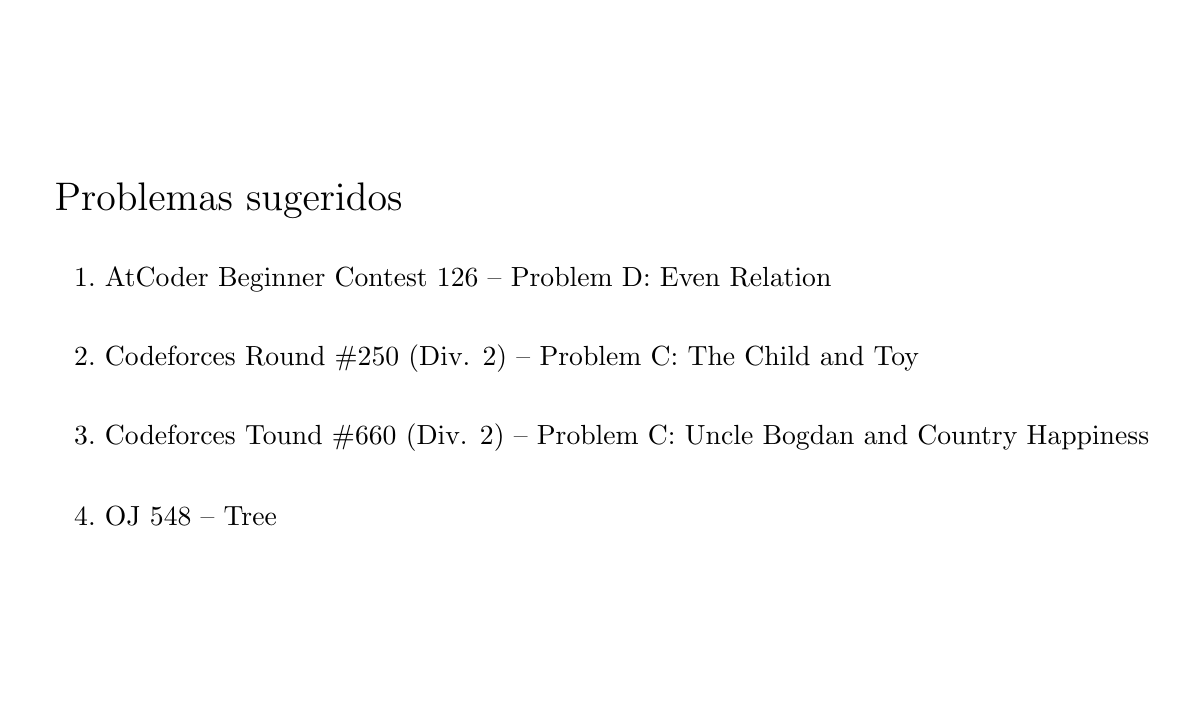
\begin{tikzpicture}
\node[draw,opacity=0] at (0, 0) {x};
\node[draw,opacity=0] at (14, 8) {x};

	\node[anchor=west] (title) at (0.0, 6.0) { \Large \bbbold{Problemas sugeridos} };

	\node[anchor=west] (a) at (0.25, 5.0) { $1.$ \bbtext{AtCoder Beginner Contest 126 -- Problem D: Even Relation} };

	\node[anchor=west] (b) at (0.25, 4.0) { $2.$ \bbtext{Codeforces Round \#250 (Div. 2) -- Problem C: The Child and Toy} };

	\node[anchor=west] (c) at (0.25, 3.0) { $3.$ \bbtext{Codeforces Tound \#660 (Div. 2) -- Problem C: Uncle Bogdan and Country Happiness} };

	\node[anchor=west] (d) at (0.25, 2.0) { $4.$ \bbtext{OJ 548 -- Tree} };

\end{tikzpicture}
\end{frame}
\begin{frame}[plain,t]

\begin{tikzpicture}
\node[draw,opacity=0] at (0, 0) {x};
\node[draw,opacity=0] at (14, 8) {x};

	\node[anchor=west] (title) at (0.0, 7.0) { \Large \bbbold{Referências} };

	\node[anchor=west] (a) at (1.0, 2.0) { $5.$ \bbtext{\bbbold{Wikipédia}. \bbenglish{Tree (graph theory),} acesso em 06/08/2021.} };

	\node[anchor=west] (e) at (1.0, 6.0) { $1.$ \bbbold{DROZDEK}, \bbtext{Adam}. \bbenglish{Algoritmos e Estruturas de Dados em C++,} \bbtext{2002.} };


	\node[anchor=west] (b) at (1.0, 5.0) { $2.$ \bbbold{HALIM}, \bbtext{Felix}; \bbbold{HALIM}, \bbtext{Steve}. \bbenglish{Competitive Programming 3,} \bbtext{2010.} };

	\node[anchor=west] (c) at (1.0, 4.0) { $3.$ \bbbold{LAAKSONEN}, \bbtext{Antti}. \bbenglish{Competitive Programmer's Handbook,} \bbtext{2018.} };

	\node[anchor=west] (d) at (1.0, 3.0) { $4.$ \bbbold{SKIENA}, \bbtext{Steven}; \bbbold{REVILLA}, \bbtext{Miguel}. \bbenglish{Programming Challenges,} \bbtext{2003.} };

\end{tikzpicture}
\end{frame}
\end{document}
